\documentclass[preprint,11pt]{elsarticle}

\usepackage[utf8]{inputenc}
\usepackage[T1]{fontenc}
\usepackage{amsmath,amssymb}
\usepackage{bm}
\usepackage{booktabs}
\usepackage{array}
\usepackage{tabularx}
\usepackage{multirow}
\newcolumntype{L}[1]{>{\raggedright\arraybackslash}p{#1}}
\newcolumntype{C}[1]{>{\centering\arraybackslash}p{#1}}
\newcolumntype{Y}{>{\raggedright\arraybackslash}X}
\usepackage{graphicx}
\usepackage{xcolor}
\usepackage{tikz}
\usepackage{pgfplots}
\pgfplotsset{compat=1.17}
\usepgfplotslibrary{groupplots}
\usetikzlibrary{arrows.meta,positioning,fit,backgrounds,calc,shapes.geometric}
\usepackage{hyperref}
\usepackage{xurl}%
\emergencystretch=1em%

\makeatletter
\def\ps@pprintTitle{\let\@oddhead\@empty\let\@evenhead\@empty
  \def\@oddfoot{}\let\@evenfoot\@oddfoot}
\makeatother

\definecolor{qpurple}{RGB}{106,61,154}
\definecolor{qblue}{RGB}{31,119,180}
\definecolor{qgreen}{RGB}{44,140,80}
\definecolor{qorange}{RGB}{214,118,32}
\definecolor{qgray}{RGB}{90,90,90}
\definecolor{lightq}{RGB}{233,226,245}
\definecolor{lightc}{RGB}{223,238,247}
\definecolor{cvviolet}{HTML}{4A3AA7}
\definecolor{cvorange}{HTML}{EB6834}
\definecolor{cvaqua}{HTML}{1BAF7A}
\definecolor{cvblue}{HTML}{2A78D6}

\newcommand{\tpr}{\mathrm{TPR}}
\newcommand{\fpr}{\mathrm{FPR}}


\begin{document}

\begin{frontmatter}

\title{How Quantum Is the Advantage? A Fair, Calibration- and Noise-Aware
Benchmark and Attribution Audit of Quantum Machine Learning for Network
Intrusion Detection}

\author[hei]{Syeda Anshrah Gillani\corref{cor1}\fnref{eq}}
\ead{syeda.gilani@stud.uni-heidelberg.de}
\author[fan]{Mirza Samad Ahmed Baig\corref{cor1}\fnref{eq}}
\ead{Mirza@fandaqah.com}
\author[sza]{Shahid Munir Shah}
\ead{dr.shahid@ghr.szabist.edu.pk}
\author[arg]{Abdul Akbar Khan}
\ead{Akbar.khan@Argaam.com}
\author[fort]{Muhammad Omer Khan}
\ead{Omer.khan@Fortanixor.com}
\author[fan]{Asher Ali}
\ead{CTO@fandaqah.com}
\author[fan]{Hamzah Siddiqui}
\ead{Hamzah@fandaqah.com}
\cortext[cor1]{Corresponding authors.}
\fntext[eq]{Syeda Anshrah Gillani and Mirza Samad Ahmed Baig are the core
contributors and contributed equally to this work.}
\address[hei]{Heidelberg University, Heidelberg, Germany}
\address[fan]{Fandaqah, Al Khobar, Saudi Arabia}
\address[sza]{Shaheed Zulfiqar Ali Bhutto Institute of Science and Technology, Karachi, Pakistan}
\address[arg]{Argaam Investment, Riyadh, Saudi Arabia}
\address[fort]{Fortanixor, Dubai, United Arab Emirates}

\begin{abstract}
A quantum-kernel advantage that survives both false-discovery-rate and family-wise correction can be
produced entirely by the tuning of the classical baseline. We show this on network intrusion detection,
where quantum machine learning routinely reports near-perfect accuracy. Benchmarking hybrid variational
circuits and quantum-kernel SVMs against five tuned classical baselines on four NIDS datasets under one
leakage-controlled protocol, with a quantum-attribution audit of parameter-matched controls, we find that
tuned classical models match or exceed the quantum models on aggregate detection on every dataset, yet a
quantum kernel significantly out-ranks its classical surrogate. With exact kernels on identical data,
the gap is set by the classical bandwidth grid: under NSL-KDD's shift to 17 unseen
attack types, in-distribution cross-validation cannot rank bandwidths, so a narrow grid yields a spurious
ROC-AUC advantage of $0.167$ while a wide grid leaves $0.007$, with the classical kernel ahead at $1\%$
false positives. On UNSW-NB15, which has no unseen attack types, standard selection is reliable and
classical kernels win outright, and holding whole attack families out of its training data recreates
the failure on demand. Leave-attack-types-out cross-validation repairs selection on NSL-KDD but not
under that induced shift, so no training-only rule is a general remedy. The geometric difference of
Huang et al.\ places the IQP kernel within $1.4$ to $2.4$ of a classical kernel on the circuit's own
phases on all four datasets. On three IBM Heron processors the projected kernel's classifier stays
within $0.01$ ROC-AUC of its exact simulation, and the four-qubit hybrid's one surviving result, higher
detection than a tuned Random Forest at $1\%$ false positives, reproduces on every device. Significance
is not attribution. Code, seeds, splits and raw device measurements are released.
\end{abstract}

\begin{keyword}
quantum machine learning \sep network intrusion detection \sep hybrid
quantum-classical neural networks \sep quantum support vector machine \sep NISQ
\sep reproducible benchmark \sep class imbalance \sep model calibration
\end{keyword}

\end{frontmatter}

\section{Introduction}
Network intrusion detection systems (NIDS) are a frontline defence against an expanding
and increasingly automated threat landscape. Machine learning has become the dominant
paradigm for flow- and packet-level intrusion detection, and the recent emergence of
quantum machine learning (QML) has prompted a fast-growing body of work applying
parameterised quantum circuits, quantum-kernel methods, and hybrid quantum-classical
neural networks to the NIDS task. Headline results are striking: accuracies and F1 scores
in the $97$ to $99.9\%$ range are reported across many datasets and quantum architectures.

These numbers invite a question the field has not answered convincingly: \textbf{how
quantum is the reported advantage?} There are three reasons for scepticism, each grounded
in rigorous recent work. First, the strongest quantum results are typically obtained on
heavily dimensionality-reduced inputs, frequently one feature per qubit after principal
component analysis (PCA), and on binary tasks evaluated under random cross-validation, a
regime that systematically over-states real-world detection. Second, when honest, well-tuned
classical baselines (Random Forests, gradient-boosted trees, modern deep networks) are placed
on the \emph{same} footing, they repeatedly match or beat the quantum models on tabular IDS
data: the Meta-Quantum Ensemble study of Bhatnagar et al.~\cite{bhatnagar2026mqe}, despite
assembling the most rigorous evaluation in the field, explicitly concedes that classical
ensembles remain superior. Third, and most pointedly, Bellante
et al.~\cite{bellante2025pca} demonstrate that the apparent advantage of
PCA-based quantum IDS is \emph{explainable by regularisation, not by quantum effects}. A
reviewer of any new QML-IDS paper will, and should, raise this point.

We take this scepticism as the starting point rather than something to argue away. A paper
whose central claim is ``our quantum model achieves higher accuracy'' is both scientifically
fragile and strategically weak, because three Q1 papers already supply the counter-argument.
The community's actual deficit is not another accuracy record; it is a \textbf{fair,
reproducible, and honest evaluation methodology}, together with a principled way to
\textbf{attribute} any measured difference to its true cause. This paper supplies both.

We construct a single, leakage-controlled benchmarking protocol and apply it to the two
quantum families that dominate the literature, namely hybrid variational quantum circuits (VQCs)
and quantum-kernel support vector machines (QSVMs), against a slate of honestly tuned
classical baselines, across four standard datasets. We honour each dataset's intended
evaluation semantics: for NSL-KDD we use the official \texttt{KDDTrain+}/\texttt{KDDTest+}
split, whose test set deliberately over-represents attack behaviour under-seen in training,
so that what we measure is generalisation to novel attacks rather than memorisation. We then
go beyond benchmarking with a \textbf{quantum-attribution audit}: for every quantum model we
construct a parameter-matched classical control sharing the identical classical front-end, and
we run a regularisation sweep that tests the Bellante et al.\ hypothesis directly. Finally,
because operational IDS must run at a low false-positive operating point and real quantum
devices are noisy, we characterise how detection and calibration behave under simulated NISQ
noise. Last, we dissect the audit's strongest positive at the level of the kernels themselves, and
show that it was produced by the tuning of the classical baseline under a distribution shift that
standard cross-validation cannot see, rather than by the quantum state.

\subsection{Contributions}
\begin{enumerate}\itemsep2pt
\item \textbf{A fair, reproducible, multi-dataset QML-IDS benchmark.} We evaluate hybrid VQCs
and QSVMs against five honestly-tuned classical baselines (Random Forest, XGBoost, RBF-SVM, a
tuned MLP, a 1D-CNN) across four standard datasets (NSL-KDD, UNSW-NB15, CICIDS2017,
NF-ToN-IoT-v2) on the binary detection task, under one protocol with strict leakage control,
honouring official splits. All code, seeds, and splits are released.
\item \textbf{An equal-budget fairness design.} We report two explicitly-labelled feature
views, a \emph{full} view (classical models on all features) and a \emph{same-budget} view
(every model on the identical low-dimensional input the quantum models receive), eliminating
the silent feature-budget asymmetry that confounds prior work.
\item \textbf{A quantum-attribution audit.} Parameter-matched classical controls and a
regularisation sweep decompose any observed gain into its quantum and classical components, a
direct constructive test of the Bellante et al.\ critique in the practical NISQ regime.
\item \textbf{A kernel-level dissection of the audit's strongest positive.} Placing quantum and
classical kernels on identical data with exact Gram matrices and equal tuning, we show that a
quantum-kernel advantage surviving both FDR and Holm correction is produced by the classical baseline's
bandwidth search, because in-distribution cross-validation cannot see the novel-attack shift of NSL-KDD's
official split. On UNSW-NB15, which lacks that shift, classical kernels win outright.
\item \textbf{An induced-shift test, the limits of shift-aware selection, and a label-free
dequantisation test.} Holding whole attack families out of UNSW-NB15's training data reproduces the
selection failure on demand. Leave-attack-types-out cross-validation repairs it on NSL-KDD, where the
unseen attacks are variants of seen families, but not under the induced shift, so we recommend reporting
kernel comparisons under several selection rules with the oracle bound. The geometric difference of
Huang et al., computed on all four datasets, shows the IQP kernel to be reproducible by a classical
kernel on its own circuit phases; the projected kernel proves robust to finite-shot measurement and, on
three IBM Heron processors, to real device noise, and the four-qubit hybrid's low-false-positive result,
the audit's one surviving positive, reproduces on the same three devices.
\item \textbf{Operationally meaningful evaluation under noise.} Beyond accuracy/F1 we report
detection rate and false-positive rate together, low-FPR operating points, and calibration, and
characterise degradation under depolarising, amplitude-damping, phase-damping, and readout-error
channels.
\item \textbf{Statistical rigour and honest framing.} Every result is a mean over three to five
seeds with confidence intervals, and we report the per-class seed budget explicitly
(Section~\ref{sec:metrics}); quantum-vs-best-classical comparisons are paired over the seeds the two
models share and use McNemar's test, paired $t$/Wilcoxon tests, and a paired bootstrap with effect
sizes. The benchmark's value does not depend on the quantum models winning.
\end{enumerate}

\section{Related Work}
We organise the related work into five strands and summarise representative studies in
Table~\ref{tab:related}.

\paragraph{Foundational and breadth-oriented QML-IDS.}
Quantum intrusion detection was established by Kalinin and Krundyshev~\cite{kalinin2022}, who
applied a quantum SVM and quantum convolutional network to a custom IoT stream dataset
($\sim$98\% accuracy); Gong et al.~\cite{gong2024vqcnn} produced the most prominent Q1
variational result (97.21\% precision, VQCNN, KDD/NSL-KDD). The strongest \emph{comparative}
line is Abreu et al.: QML-IDS~\cite{abreu2024qmlids} and QuantumNetSec~\cite{abreu2025quantumnetsec}
span VQC, QSVM, and QCNN across three to four datasets, but with under-tuned classical baselines
and no attribution of where gains originate.

\paragraph{Methods landscape.}
The dominant primitive is the parameterised quantum circuit used as a variational classifier or
hybrid head; recurring concerns are trainability (barren plateaus) and encoding choice, with
amplitude embedding reported as unstable relative to angle embedding~\cite{wang2025quanconv}.
Quantum-kernel SVMs~\cite{kumari2025wavelet} form the second family, scaling poorly in sample
count, hence the reliance on subsampled, PCA-reduced data. Newer directions include quantum GNNs
(Q-AGNN~\cite{chaudhary2026qagnn}) and meta-learning ensembles~\cite{bhatnagar2026mqe}.

\paragraph{Rigorous and sceptical evaluations.}
A small set of studies interrogates whether quantum helps. Bhatnagar et al.'s Meta-Quantum
Ensemble~\cite{bhatnagar2026mqe} sets the field's evaluation standard (AUPRC, $\tpr$ at low
$\fpr$, Brier, ECE, five noise channels) yet concludes classical ensembles remain superior.
Bellante et al.~\cite{bellante2025pca}, in \emph{Computers \& Security}, show the observed
advantage is explainable by regularisation rather than quantum effects. These works define the
bar we must clear: not a higher accuracy, but a fair and \emph{attributable} comparison.

\paragraph{Quantum kernels under scrutiny.}
Outside intrusion detection, a growing literature asks the same question of quantum kernels. Schnabel
and Roth~\cite{schnabel2025scrutiny} benchmark fidelity and projected quantum kernels over 64 datasets and
more than 20{,}000 models, and find that classical hyperparameters, notably regularisation and bandwidth,
matter more than the number of qubits or layers, with no substantial difference between fidelity and
projected kernels. Fl\'orez-Ablan et al.~\cite{florezablan2025similarity} show that optimally bandwidth-tuned
quantum kernels closely resemble RBF kernels and so hold no quantum advantage, and Shaydulin and
Wild~\cite{shaydulin2022bandwidth} establish the importance of the bandwidth itself. Kakavand
et al.~\cite{kakavand2026benchmarking} find no significant advantage for quantum-kernel SVMs across nine
tabular datasets, with hardware validation. Abdulsalam and Ahmad~\cite{abdulsalam2025comparative}
compare fidelity quantum kernels with RBF, linear, polynomial and sigmoid kernels, in both classical and
quantum SVMs, across eleven tabular classification and regression datasets, and Innan
et al.~\cite{innan2023variational} train the quantum kernel variationally to improve QSVM accuracy.
Huang et al.~\cite{huang2021power} supply a label-free criterion, the geometric difference, for when a
quantum kernel can outperform a classical one at all.
To our knowledge none of these studies examines the novel-attack shift between training and test data
that defines NIDS evaluation. Within intrusion detection, Cotrupi and Callahan~\cite{cotrupi2025practical}
run quantum kernels on hardware for four attack types, reporting an average accuracy of 85\%. We extend
this line to that shift, and show how it interacts with the tuning of the classical baseline.

\paragraph{Datasets and evaluation practice.}
Most studies use one or two datasets (NSL-KDD/KDD99 the dated-but-default choice); genuine
multi-dataset and cross-dataset evaluation is rare, and imbalance-aware metrics, calibration,
significance testing, and honest baselines are almost universally missing, with
Bhatnagar et al.~\cite{bhatnagar2026mqe} the principal exception.

\begin{table}[t]
\centering
\caption{Representative QML-IDS studies and where this work differs (``sim''~=~simulator).}
\label{tab:related}
\footnotesize
\renewcommand{\arraystretch}{1.2}
\setlength{\tabcolsep}{3pt}
\begin{tabularx}{\textwidth}{@{}L{2.25cm} L{2.1cm} Y C{1.85cm} C{1.95cm}@{}}
\toprule
\textbf{Paper} & \textbf{Method} & \textbf{Dataset(s)} & \textbf{Honest baseline?} & \textbf{Attribution?}\\
\midrule
Kalinin \& Krundyshev \cite{kalinin2022} & QSVM, QCNN & Custom IoT stream & No & No\\
\addlinespace[2pt]
Gong et al.~\cite{gong2024vqcnn} & VQCNN & KDD / NSL-KDD & Partial & No\\
\addlinespace[2pt]
Abreu et al.~\cite{abreu2024qmlids,abreu2025quantumnetsec} & VQC / QSVM / QCNN & UNSW, CICIDS, CIC-IoT & Under-tuned & No\\
\addlinespace[2pt]
Bhatnagar et al.~\cite{bhatnagar2026mqe} & QSVM, QNN, RF & CICIDS, TON\_IoT & Yes (cl.\ wins) & No\\
\addlinespace[2pt]
Bellante et al.~\cite{bellante2025pca} & FT PCA-QML & NIDS datasets & Yes & FT/PCA only\\
\addlinespace[2pt]
\textbf{This work} & VQC, QSVM, controls & 4 datasets, official splits & Yes (5 tuned) & Yes (NISQ)\\
\bottomrule
\end{tabularx}
\end{table}

We differentiate on three axes. Against Abreu et al.\ we retain breadth but add tuned baselines,
an equal-budget view, operating-point and calibration metrics, significance testing, and
reproducibility. Against Bhatnagar et al.\ we add the causal \emph{decomposition} their paper
concedes is missing. Against Bellante et al., the sharpest existing critique of PCA-based
quantum IDS, we
extend the regularisation argument from their fault-tolerant, PCA-specific case study to the
practical NISQ hybrid-VQC and QSVM models the community deploys, across a full multi-dataset
benchmark, and we do so constructively: we specify exactly what evidence a genuine advantage would
require and report whether, where, and to what extent it appears.

\section{Threat Model and Background}
\subsection{Threat model}
We consider flow- and connection-record-based detection: a model classifies each per-connection
feature vector as benign or malicious. Three operational constraints shape the evaluation: a strong
\emph{cost asymmetry} (false positives flood analysts, so a detector must hold up at a low-$\fpr$
operating point); \emph{distribution shift} between training and deployment, including unseen attack
signatures (why we honour the NSL-KDD official split); and \emph{class imbalance}. Adaptive
adversarial evasion is out of scope.

\subsection{Background on quantum machine learning}
A QML model operates on $n$ qubits whose joint state is a unit vector in a $2^n$-dimensional complex
space; a noiseless simulation tracks this $2^n$-entry vector, while a noisy simulation tracks a
$2^n\times 2^n$ density matrix, whose quadratic cost caps our noisy runs at twelve qubits. Classical
flow features must be \emph{encoded} into the circuit (we ablate angle, amplitude, IQP/ZZ, and
data-re-uploading encodings); a \emph{variational} ansatz of trainable gates processes the state; and
measured Pauli-$Z$ expectations are mapped to class logits by a classical layer
(Figure~\ref{fig:arch}). An alternative is to use the circuit only as a fixed feature map and let a
classical SVM learn the boundary: the \emph{fidelity kernel} $K(x,x')=|\langle\phi(x')|\phi(x)\rangle|^2$
costs $O(N^2)$ circuit evaluations, while the \emph{projected kernel} computes per-qubit expectations
and applies a classical RBF, scaling as $O(N)$.

The link to our central question is direct: in every hybrid pipeline a \emph{classical} front-end
compresses high-dimensional records to the per-qubit budget and a \emph{classical} read-out turns
measurements into predictions, so any end-to-end accuracy blends a quantum contribution with
substantial classical processing and implicit regularisation. Disentangling the two is exactly what
the attribution audit (Section~\ref{sec:audit}) is built to do.

\begin{figure}[t]
\centering
\resizebox{\textwidth}{!}{%
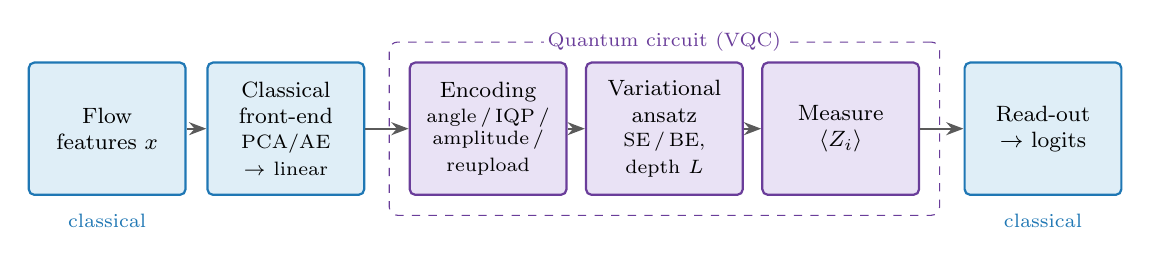
\begin{tikzpicture}[
  font=\footnotesize,
  box/.style={rounded corners=2pt,draw,thick,align=center,
              text width=1.78cm,minimum height=1.68cm,inner xsep=3pt},
  cbox/.style={box,fill=lightc,draw=qblue},
  qbox/.style={box,fill=lightq,draw=qpurple},
  arr/.style={-{Stealth[length=2.2mm]},thick,qgray},
  sub/.style={qblue,font=\scriptsize},
  ]
  \node[cbox]                      (in)   {Flow\\features $x$};
  \node[cbox,right=0.25cm of in]   (pre)  {Classical\\front-end\\[1pt]\scriptsize PCA/AE\\$\to$ linear};
  \node[qbox,right=0.55cm of pre]  (enc)  {Encoding\\[1pt]\scriptsize angle\,/\,IQP\,/\\amplitude\,/\\reupload};
  \node[qbox,right=0.22cm of enc]  (ans)  {Variational\\ansatz\\[1pt]\scriptsize SE\,/\,BE,\\depth $L$};
  \node[qbox,right=0.22cm of ans]  (meas) {Measure\\$\langle Z_i\rangle$};
  \node[cbox,right=0.55cm of meas] (out)  {Read-out\\$\to$ logits};
  \draw[arr] (in)   -- (pre);
  \draw[arr] (pre)  -- (enc);
  \draw[arr] (enc)  -- (ans);
  \draw[arr] (ans)  -- (meas);
  \draw[arr] (meas) -- (out);
  \begin{scope}[on background layer]
    \node[draw=qpurple,dashed,rounded corners=3pt,inner sep=7pt,
          fit=(enc)(ans)(meas)] (qfit) {};
  \end{scope}
  \node[qpurple,font=\scriptsize,fill=white,inner sep=1.5pt,
        anchor=center] at (qfit.north) {Quantum circuit (VQC)};
  \node[sub,below=3pt of in.south]  {classical};
  \node[sub,below=3pt of out.south] {classical};
\end{tikzpicture}}
\caption{Hybrid quantum-classical classifier. A classical front-end compresses flow features to the
per-qubit budget; a variational quantum circuit (encoding $+$ ansatz $+$ measurement) processes the
encoded state; a classical read-out produces class logits. The quantum component is sandwiched between
classical processing, which is the motivation for the attribution audit.}
\label{fig:arch}
\end{figure}

\section{Methodology}
\subsection{Benchmark protocol and leakage control}
We evaluate every model under one protocol designed so no test-distribution information influences
training, scaling, reduction, or model selection. Where a dataset ships an official split we honour
it: NSL-KDD uses the canonical \texttt{KDDTrain+}/\texttt{KDDTest+} split (17 attack signatures appear
only in test, so we measure generalisation to novel attacks); UNSW-NB15 uses its official CSVs;
CICIDS2017 and NF-ToN-IoT-v2 use a single seeded stratified $70/30$ split. All preprocessing is fit on
training data only; leaky identifier columns (IP/port four-tuples, flow IDs, timestamps, row indices)
are dropped; model selection is by cross-validation \emph{within the training set only}, and the test
set is scored once per model per seed.

\subsection{Two feature views (equal-budget fairness)}
We report a \textbf{full view} (classical baselines on all encoded dimensions, the practical ceiling)
and a \textbf{same-budget view} (every model on the identical PCA-reduced input, $n_{\text{features}}=
n_{\text{qubits}}=8$ in the main configuration). Because one-hot expansion produces many sparse columns,
standard-scaling before PCA wastes the budget (eight components retain only $\sim$27\% of variance on
NSL-KDD); min-max scaling before PCA lifts this to $0.841$ (Table~\ref{tab:data}), so we min-max scale
prior to reduction.

\subsection{Models}
The quantum side is a hybrid VQC family and two QSVMs through a single model factory: a
parameter-matched classical MLP control, six hybrid VQCs over the encoding~$\times$~ansatz grid
(angle, IQP/ZZ, amplitude, re-uploading; strongly-entangling [SE] and basic-entangler [BE] ans\"atze),
and two QSVMs (IQP fidelity-kernel, angle projected-kernel). The ZZ feature map is built from primitive
gates for correct mini-batch broadcasting. The five classical baselines (Random Forest, XGBoost,
RBF-SVM, tuned MLP, 1D-CNN) are each hyperparameter-searched (randomised search / grid, 5-fold
stratified CV on the training set, optimising F1) and refit per seed.

\subsection{The quantum-attribution audit}\label{sec:audit}
This is the methodological core and our constructive answer to Bellante et al.~\cite{bellante2025pca}.
Figure~\ref{fig:audit} sketches the logic. The audit has three components: (i) \emph{parameter-matched
classical controls}: for each hybrid VQC, a classical MLP of matched parameter count sharing the
identical front-end, and for each QSVM an RBF-SVM and a \emph{random-feature} kernel approximation; if a
matched control equals the quantum model, the ``advantage'' is not attributable to the quantum component;
(ii) a \emph{regularisation sweep} varying classical regularisation (read-out ridge, MLP weight decay,
RF depth, SVM bandwidth) to test whether comparable regularisation closes any gap; and (iii) a \emph{gain
decomposition} reporting, per dataset and metric, the quantum-minus-control difference with significance.

\begin{figure}[t]
\centering
\resizebox{0.95\textwidth}{!}{%
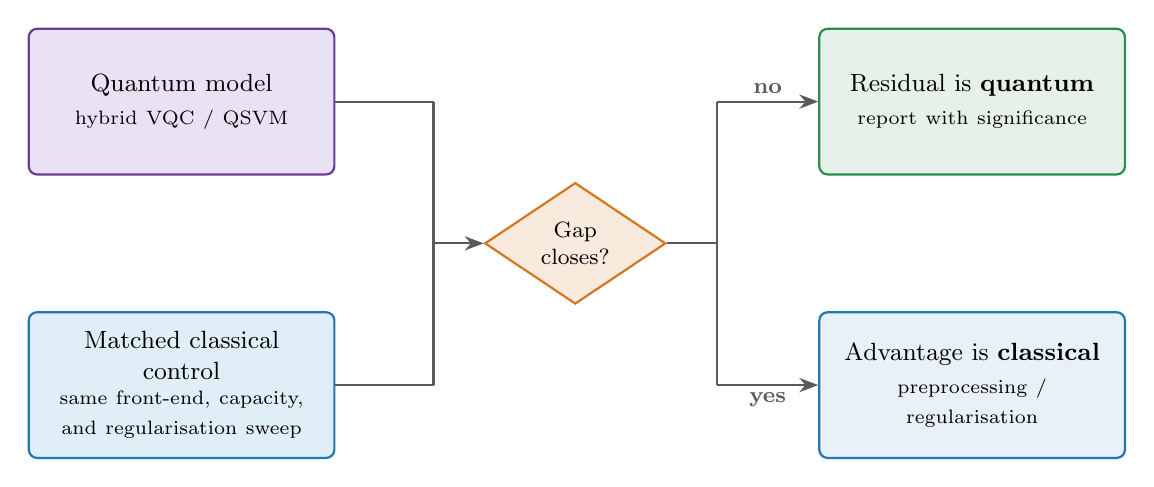
\begin{tikzpicture}[
  font=\small,
  bx/.style={rounded corners=3pt,draw,thick,align=center,
             text width=3.6cm,minimum height=1.85cm,inner xsep=4pt},
  qb/.style={bx,draw=qpurple,fill=lightq},
  cb/.style={bx,draw=qblue,fill=lightc},
  res/.style={bx,draw=qgreen,fill=qgreen!12},
  cl/.style={bx,draw=qblue,fill=qblue!10},
  dec/.style={diamond,draw=qorange,thick,fill=qorange!15,align=center,
              inner sep=1pt,minimum width=2.3cm,minimum height=1.4cm,
              font=\footnotesize},
  ln/.style={thick,qgray},
  arr/.style={ln,-{Stealth[length=2.4mm]}},
  lbl/.style={font=\footnotesize\bfseries,fill=white,inner sep=1.5pt},
  ]
  \node[qb] (q)   at (0, 1.8) {Quantum model\\[1pt]\scriptsize hybrid VQC / QSVM};
  \node[cb] (c)   at (0,-1.8) {Matched classical\\control\\[1pt]\scriptsize same front-end, capacity,\\and regularisation sweep};
  \node[dec] (d)  at (5.0, 0)  {Gap\\closes?};
  \node[res] (qu)  at (10.04, 1.8) {Residual is \textbf{quantum}\\[1pt]\scriptsize report with significance};
  \node[cl]  (cla) at (10.04,-1.8) {Advantage is \textbf{classical}\\[1pt]\scriptsize preprocessing / regularisation};
  \draw[ln]  (q.east) -- (3.2, 1.8);
  \draw[ln]  (c.east) -- (3.2,-1.8);
  \draw[ln]  (3.2,1.8) -- (3.2,-1.8);
  \draw[arr] (3.2,0) -- (d.west);
  \draw[ln]  (d.east) -- (6.8,0);
  \draw[ln]  (6.8,1.8) -- (6.8,-1.8);
  \draw[arr] (6.8, 1.8) -- node[lbl,pos=0.5,above=1pt] {no}  (qu.west);
  \draw[arr] (6.8,-1.8) -- node[lbl,pos=0.5,below=1pt] {yes} (cla.west);
\end{tikzpicture}}
\caption{The attribution audit. Each quantum model is compared with a parameter-matched classical
control sharing its front-end, plus a regularisation sweep. If a comparably-regularised classical model
closes the gap, the apparent advantage is classical; any significant residual is attributed to the
quantum circuit.}
\label{fig:audit}
\end{figure}

\subsection{Kernel-level diagnostics}\label{sec:kdiag}
The audit above compares models. To explain \emph{why} a quantum kernel does or does not help, we also
analyse the kernels themselves. Every quantum kernel studied here is noiseless, so we simulate each
feature-map state $|\phi(x)\rangle$ once and form every Gram matrix from the stored statevectors: the
fidelity kernel as $|\Psi_A\Psi_B^{\dagger}|^{2}$, and the projected kernel from each qubit's reduced
density matrix. This costs $O(N)$ circuit simulations instead of $O(N^{2})$, a shortcut available only in simulation, agrees with the circuits
used for the QSVM to within $10^{-15}$ on every entry, and reproduces the published QSVM test metrics to
four decimal places.

\paragraph{Fair surrogates.} We compare quantum and classical kernels on the identical first 2{,}000
NSL-KDD training rows, with exact Gram matrices and the same kernel SVM solver throughout. The bandwidth $\gamma$ and
$C\in\{0.1,1,10,100\}$ are selected on the training rows only, with the same grid for quantum and
classical kernels, so neither side receives more tuning than the other. We use two bandwidth grids,
because the choice matters: a narrow one of seven values from $0.003$ to $3$, and a wide one of ten
values from $0.001$ to $30$, both logarithmically spaced. Selection is either standard 5-fold
stratified cross-validation or the shift-aware variant described in Section~\ref{sec:kcv}.

\paragraph{Induced shift.} To test whether novel attack types cause the selection failure rather than
merely accompany it, we repeat the kernel comparison on UNSW-NB15 after removing whole attack categories
from the training sample while leaving them in the test sample, with two different sets of removed
categories (Section~\ref{sec:kinduced}). As a sensitivity check on the shift-aware rule we also report a
second fold construction, which splits benign rows evenly across folds and assigns attack types
largest-first to the fold holding the fewest attack rows, so that every fold contains both classes.

\paragraph{Geometric difference and model complexity.} Following Huang et al.~\cite{huang2021power}, for
kernels normalised to $\operatorname{Tr}K=N$ we compute
\[
g(K_C\Vert K_Q)=\sqrt{\Bigl\Vert\sqrt{K_Q}\,\sqrt{K_C}\,(K_C+\lambda I)^{-2}\sqrt{K_C}\,\sqrt{K_Q}\Bigr\Vert_{\infty}},
\]
which tends to $\sqrt{\Vert\sqrt{K_Q}K_C^{-1}\sqrt{K_Q}\Vert_{\infty}}$ as $\lambda\to 0$. A small $g$
certifies that the classical kernel can learn any function the quantum kernel can learn from comparable
data, for \emph{any} labelling of the inputs, whereas a prediction advantage requires $g$ to approach
$\sqrt{N}$. We take the minimum of $g$ over each classical kernel family and bandwidth, at $N=800$ and
$\lambda=10^{-2}$. Rank-deficient kernels, such as the linear kernel on eight features, are excluded:
their regularised inverse vanishes on the null space, which makes $g$ spuriously small. We also report
the label-dependent model complexity $s_K=\Vert\sqrt{K}(K+\lambda I)^{-1}y\Vert^{2}$ with $y\in\{\pm1\}$,
which tends to $y^{\top}K^{-1}y$ as $\lambda\to 0$.

\paragraph{Concentration.} We measure the mean and variance of the off-diagonal kernel entries as the
qubit count grows from 2 to 12. Exponential concentration~\cite{thanasilp2024concentration} would drive
this variance to zero exponentially in the number of qubits.

\paragraph{Finite shots.} Each Pauli expectation $\mu$ in the projected kernel is replaced by the mean of
$M$ outcomes in $\{\pm1\}$ drawn with $P(+1)=(1+\mu)/2$, which is what hardware returns from $M$ shots in
each of the three measurement bases, and the SVM is retrained on the resulting noisy features.

\paragraph{Hardware execution.} Because the projected kernel needs only single-qubit expectations, the
feature map can be run on a real device as one parameterised eight-qubit circuit with 24 observables,
executed once per sample: linear in the number of samples, unlike the $O(N^{2})$ fidelity kernel. We
build the identical IQP circuit in Qiskit (its statevector expectations agree with the PennyLane feature
map to $10^{-15}$), transpile it to the device's native gate set (depth 119, 28 two-qubit gates on the
heavy-hex coupling map), and evaluate $\langle X_i\rangle,\langle Y_i\rangle,\langle Z_i\rangle$ with the
Estimator primitive at 128 shots per measurement basis, with the primitive's default readout-error
mitigation and no other error mitigation. The 200 training rows are the first 200 of the NSL-KDD training
file and the 500 test rows are a seeded, class-balanced sample of the official test set. All 700 samples
are submitted as a single job. We compare the measured features and the resulting Gram matrix with their
exact statevector values by Pearson correlation, and train and test the projected-kernel SVM on the
measured features alone. As a control we first run the same pipeline on a noisy local simulation of the
device built from its calibration data.

The same devices also run the variational model behind the audit's one surviving positive, the
four-qubit hybrid of Table~\ref{tab:audit}. Its trained circuit (angle encoding, three strongly
entangling layers) is rebuilt in Qiskit with the trained weights bound as constants and the four input
angles as circuit parameters (statevector expectations agree with PennyLane to $10^{-15}$), transpiled to
the heavy-hex coupling map (depth 81 to 92 and 21 to 30 two-qubit gates, depending on the layout chosen
for the device's current calibration), and its four $\langle Z_i\rangle$ are measured at 128 shots for a
seeded, class-balanced sample of 2{,}000 test rows, as one job per device. The measured expectations pass
through the trained classical head unchanged, so only the quantum layer is replaced. The model is
retrained from the released configuration and seed before the run; the retrained model reproduces the
published test scores to $2\times10^{-8}$. We compare it with the tuned Random Forest of
Table~\ref{tab:audit} on the same 2{,}000 rows by paired bootstrap.

\paragraph{Classical phase kernels.} Under angle encoding every qubit remains in a product state, so its
Pauli features are exactly $(\sin x_i, 0, \cos x_i)$ and the ``quantum'' projected kernel is an RBF kernel
on classical trigonometric features. We therefore also test RBF kernels on
$\varphi(x)=(\sin x_i,\cos x_i)_{i}$, and on $\varphi$ augmented with the phases that the ZZ feature
map~\cite{havlicek2019supervised} writes into the state, namely $\sin$ and $\cos$ of $2x_i$ and of
$2(\pi-x_i)(\pi-x_{i+1})$. This isolates whether an advantage requires the quantum state itself, or only
the phases it encodes.

\subsection{Class imbalance and noise}
The NSL-KDD binary task is only mildly imbalanced, so we default to cost-sensitive learning (balanced
class weights, \texttt{scale\_pos\_weight} for XGBoost, weighted cross-entropy) and treat SMOTE
(training partition only) as an ablation. For noise robustness we sweep four channels (depolarising,
amplitude damping, phase damping, and bit-flip readout) at strengths $p\in\{0,0.001,0.005,0.01,0.05\}$
on PennyLane's \texttt{default.mixed} density-matrix backend, capped at twelve qubits.

\section{Experimental Setup}
\subsection{Datasets}
We evaluate on four standard NIDS datasets (Table~\ref{tab:data}). The \textbf{main benchmark is the
binary task}. CICIDS2017 here is the three-day \emph{MachineLearningCVE} subset ($\sim$1.04M flows);
NF-ToN-IoT-v2 is stratified-downsampled to 200{,}000 rows (from 16.9M); both are standard, configurable
scopes we disclose plainly.

\begin{table}[t]
\centering
\caption{Datasets (binary task; PCA-EVR@8 = variance retained by 8 principal components).}
\label{tab:data}
\footnotesize
\renewcommand{\arraystretch}{1.15}
\setlength{\tabcolsep}{4pt}
\begin{tabular}{@{}llcccc@{}}
\toprule
\textbf{Dataset} & \textbf{Split} & \textbf{Raw} & \textbf{Classes} & \textbf{Train / test} & \textbf{EVR@8}\\
                 &                & \textbf{dim} & \textbf{(bin / multi)} & & \\
\midrule
NSL-KDD~\cite{nslkdd2009}    & Official      & 122 & 2 / 40 & 125{,}973 / 22{,}544  & 0.841\\
UNSW-NB15~\cite{unswnb15}    & Official      & 194 & 2 / 10 & 175{,}341 / 82{,}332  & 0.870\\
CICIDS2017~\cite{cicids2017} & Strat.\ 70/30 &  76 & 2 / 3  & 729{,}491 / 312{,}639 & 0.924\\
NF-ToN-IoT-v2~\cite{toniot}  & Strat.\ 70/30 &  39 & 2 / 10 & 140{,}000 / 60{,}000  & 0.974\\
\bottomrule
\end{tabular}
\end{table}

\subsection{Metrics and significance}\label{sec:metrics}
We report threshold metrics (accuracy, precision, recall, F1, detection rate DR, false-positive rate
$\fpr$) and ranking/calibration metrics (ROC-AUC, AUPRC, $\tpr$@$0.1\%\fpr$, $\tpr$@$1\%\fpr$, Brier,
ECE), matching and extending the Meta-Quantum-Ensemble suite~\cite{bhatnagar2026mqe}. We state the
seed budget exactly, because it is uneven across model classes. The tuned classical baselines are run
over five seeds $\{42,43,44,45,46\}$ on NSL-KDD and over three seeds $\{42,43,44\}$ on UNSW-NB15,
CICIDS2017 and NF-ToN-IoT-v2; the quantum models and the attribution-audit controls over three seeds
$\{42,43,44\}$; and the noise-robustness sweep over two seeds $\{42,43\}$, with all RNGs pinned per
seed and $t$-based 95\% confidence intervals reported throughout. Every quantum-versus-classical
comparison is therefore paired over the three seeds $\{42,43,44\}$ that all models share, and uses
McNemar's
test (shared test set), paired $t$/Wilcoxon tests with Cohen's $d$ (over seeds), and a paired bootstrap
(2{,}000 resamples) for operating-point metrics. Because the attribution audit evaluates many
variant$\times$metric comparisons, we control the false-discovery rate across this family with the
Benjamini-Hochberg (BH) procedure and report BH-adjusted $q$-values alongside raw $p$-values; we treat
a result as robust only if it survives FDR control.

\subsection{Backend efficiency and reproducibility}
At QML-IDS qubit counts, quantum simulation (not GPU throughput) dominates runtime, and we report a
\textbf{backend crossover}: the CPU \texttt{lightning.qubit} simulator is markedly faster than the GPU
\texttt{lightning.gpu} simulator (Section~\ref{sec:eff}). Each run writes a self-describing JSON record
(config, per-seed metrics, tuned hyperparameters, reference-seed predictions, environment snapshot with
source checksums). All experiments run on a single laptop (NVIDIA RTX~3050~Ti, 4\,GB, under WSL2); the
main runs use eight qubits, with a ceiling of sixteen (noiseless) / twelve (noisy). Code, seeds, and
splits are released.

\section{Results}
The overall result, qualified below: \emph{honestly-tuned classical models match or exceed the quantum
models on aggregate detection on every dataset, but a small hybrid VQC retains a statistically
significant edge at the strict low-$\fpr$ operating point on the distribution-shifted NSL-KDD task.}

\subsection{Headline benchmark}
Table~\ref{tab:headline} reports F1 under both views. Under the \emph{same-budget} view (the
apples-to-apples comparison), the best classical baseline beats the leading 8-qubit quantum model on
every dataset: NSL-KDD $0.782$ vs.\ $0.730$; UNSW-NB15 $0.891$ vs.\ $0.836$; CICIDS2017 $1.000$ vs.\
$0.968$; NF-ToN-IoT-v2 $0.991$ vs.\ $0.949$. On NSL-KDD the strongest quantum \emph{ablation} variants
narrow this gap substantially, since the IQP-encoded QSVM and the 4-qubit hybrid reach F1 of $0.752$ and
$0.759$ (Section~\ref{sec:audit-results}), but tuned classical still leads on F1, and retains a clearer
margin on AUPRC and ROC-AUC, so the aggregate ordering is unchanged. Two qualifications
matter. First, \textbf{CICIDS2017 and NF-ToN-IoT-v2 are near-saturated} (every tuned classical model
scores F1~$\geq 0.97$), so they have weak discriminative power and the quantum models' high absolute
scores there should be read as ``this task is easy.'' Second, the \textbf{CV-to-test gap} confirms why
literature numbers are inflated: on NSL-KDD, models scoring F1~$\approx 0.98$ under within-training
cross-validation collapse to F1~$\approx 0.78$ on the official test split, a consistent $\approx 0.20$
drop across all models and both views. Figure~\ref{fig:bars} compares the best classical and best
quantum F1 per dataset; the qubit-count ablation is shown later in Figure~\ref{fig:ablation}.

\begin{table}[t]
\centering
\caption{Headline benchmark. F1 (mean over seeds): best classical per view vs.\ the leading
8-qubit quantum model per dataset (same-budget input). The final three columns give that quantum
model's AUPRC, ROC-AUC, and $\tpr$@$1\%\fpr$. Stronger quantum ablation variants (e.g.\ the IQP-QSVM
and the 4-qubit hybrid on NSL-KDD, F1 $0.752$ and $0.759$) are analysed in Section~\ref{sec:audit-results}.}
\label{tab:headline}
\small
\renewcommand{\arraystretch}{1.2}
\setlength{\tabcolsep}{5pt}
\begin{tabular}{@{}lcccccc@{}}
\toprule
& \multicolumn{2}{c}{\textbf{Classical F1}} & \multicolumn{4}{c}{\textbf{Quantum (8 qubits, same-budget)}}\\
\cmidrule(lr){2-3}\cmidrule(lr){4-7}
\textbf{Dataset} & \textbf{full} & \textbf{same-} & \textbf{F1} & \textbf{AUPRC} & \textbf{ROC-} & \textbf{TPR@}\\
                 &               & \textbf{budget} &            &                & \textbf{AUC}  & \textbf{1\%\,FPR}\\
\midrule
NSL-KDD       & 0.803 & 0.782 & 0.730 & 0.911 & 0.865 & 0.411\\
UNSW-NB15     & 0.912 & 0.891 & 0.836 & 0.942 & 0.924 & 0.577\\
CICIDS2017    & 1.000 & 1.000 & 0.968 & 0.992 & 0.998 & 0.975\\
NF-ToN-IoT-v2 & 0.996 & 0.991 & 0.949 & 0.965 & 0.969 & 0.195\\
\bottomrule
\end{tabular}

\smallskip
\begin{minipage}{\textwidth}\footnotesize\raggedright
Best classical model per cell. Full view: SVM (NSL-KDD), MLP (UNSW), RF (CICIDS, NF-ToN-IoT-v2);
same-budget: XGBoost (NSL-KDD), MLP (UNSW), RF (CICIDS, NF-ToN-IoT-v2).
\end{minipage}
\end{table}

\subsection{Attribution audit}\label{sec:audit-results}
The audit (Table~\ref{tab:audit}) decomposes the difference on NSL-KDD, the discriminative dataset. A
parameter-matched classical MLP sharing the quantum front-end attains AUPRC $0.944$ and the tuned Random
Forest attains F1 $0.764$, both matching or exceeding every hybrid VQC on aggregate metrics. For the
twelve-qubit hybrid the classical controls win significantly (F1 $-0.039$, $p=0.021$; AUPRC $-0.036$,
$p=0.035$; $\tpr$@$1\%\fpr$ $-0.121$, $p=0.026$). \textbf{Once a classical model is granted the same
front-end and comparable capacity/regularisation, the aggregate ``quantum advantage'' disappears}, a
confirmation of the Bellante hypothesis on this dataset. Two exceptions survive
Benjamini-Hochberg FDR control across the audit's comparison family, however, and they are the most
informative results in the audit. First, the quantum-kernel SVM significantly
out-performs the random-feature (Nystr\"om / RBF-sampler) kernel: on
NSL-KDD the IQP-encoded QSVM beats the random-feature control on AUPRC ($\Delta=+0.075$, raw $p=0.001$,
BH $q=0.011$), ROC-AUC ($\Delta=+0.134$, $p=0.002$, $q=0.018$), and $\tpr$@$1\%\fpr$ ($\Delta=+0.152$,
$p=0.017$, $q=0.047$). Taken at face value this would isolate a genuinely quantum contribution, since
the random-feature kernel is meant as the classical surrogate for the quantum feature map.
Section~\ref{sec:kernel} shows that it does not: the control differed from the QSVM in four further
ways, and once those are removed the gap is set by the classical bandwidth search, while a classical
kernel on the circuit's own phases reproduces the quantum kernel.
Second, the \emph{four-qubit} hybrid beats the tuned Random Forest at the low-$\fpr$ operating point
($\tpr$@$1\%\fpr$ $+0.050$, $p=0.005$, BH $q=0.030$; Section~\ref{sec:op}). The remaining quantum
differences are either ties or significant \emph{losses} to the classical controls (notably the
twelve-qubit hybrid: F1 $-0.039$, $p=0.021$; AUPRC $-0.036$, $p=0.035$), consistent with overfitting at
width rather than a quantum benefit. Within the audit, then, classical wins on aggregate and two
FDR-robust quantum differences persist: the quantum kernel over the random-feature control, which
Section~\ref{sec:kernel} traces to the control, and the small hybrid at the strict operating point.

\begin{table}[t]
\centering
\caption{Quantum-attribution audit (NSL-KDD): leading quantum variants vs.\ best matched control.
$\Delta=$ quantum $-$ control (positive favours quantum, except ECE). $q$ is the Benjamini-Hochberg
FDR-adjusted value across the audit family; \textbf{bold} rows survive FDR control ($q<0.05$).
``Hyb.-Angle q$n$'' is the angle-encoded hybrid VQC on $n$ qubits; rf-kern is the random-feature
kernel and MLP-m the parameter-matched MLP.}
\label{tab:audit}
\footnotesize
\renewcommand{\arraystretch}{1.15}
\setlength{\tabcolsep}{3pt}
\resizebox{\textwidth}{!}{%
\begin{tabular}{@{}l l c l r c r r@{}}
\toprule
\textbf{Variant} & \textbf{Metric} & \textbf{Quantum} & \textbf{Best control} & $\bm{\Delta}$ & \textbf{Q}     & $\bm{p}$ & $\bm{q}$\\
                 &                 &                  &                      &               & \textbf{better?} &          & \textbf{(BH)}\\
\midrule
\textbf{QSVM-IQP}  & \textbf{AUPRC}       & \textbf{0.957} & \textbf{0.882 (rf-kern)} & $\bm{+0.075}$ & \textbf{yes} & \textbf{0.001} & \textbf{0.011}\\
\textbf{QSVM-IQP}  & \textbf{ROC-AUC}     & \textbf{0.945} & \textbf{0.811 (rf-kern)} & $\bm{+0.134}$ & \textbf{yes} & \textbf{0.002} & \textbf{0.018}\\
\textbf{QSVM-IQP}  & \textbf{TPR@1\%FPR}  & \textbf{0.470} & \textbf{0.318 (rf-kern)} & $\bm{+0.152}$ & \textbf{yes} & \textbf{0.017} & \textbf{0.047}\\
\textbf{Hyb.-Angle q4}  & \textbf{TPR@1\%FPR} & \textbf{0.517} & \textbf{0.467 (RF)} & $\bm{+0.050}$ & \textbf{yes} & \textbf{0.005} & \textbf{0.030}\\
Hyb.-Angle q4      & TPR@0.1\%FPR         & 0.407 & 0.272 (MLP-m) & $+0.135$ & yes & 0.428 & 0.62\\
Hyb.-Angle q4      & F1                   & 0.759 & 0.764 (RF)    & $-0.004$ & tie & 0.776 & 0.84\\
Hyb.-Angle q12     & F1                   & 0.724 & 0.764 (RF)    & $-0.039$ & no  & 0.021 & 0.10\\
Hyb.-Angle q12     & TPR@1\%FPR           & 0.346 & 0.467 (RF)    & $-0.121$ & no  & 0.026 & 0.11\\
\bottomrule
\end{tabular}}
\end{table}

\subsection{Operating-point and calibration analysis}\label{sec:op}
The operating-point metrics hold one of the audit's two FDR-robust quantum differences; the other, the
quantum-kernel-vs-random-feature-kernel comparison, is analysed in Section~\ref{sec:kernel}. On NSL-KDD the
four-qubit hybrid VQC achieves $\tpr$@$1\%\fpr=0.517$, exceeding the best classical model (Random Forest,
$0.467$) by $0.050$, statistically significant ($p=0.005$, paired bootstrap). At $0.1\%\fpr$ it reaches
$0.407$ against $0.272$, a difference that is not significant ($p=0.43$). At the strict $1\%$-alarm budget
a defender would actually impose, the small quantum model catches a larger fraction of attacks on
novel-attack-heavy traffic. Calibration is comparable (ECE $\approx 0.18$ to $0.22$ for hybrids vs.\ $0.193$
for Random Forest), the four-qubit hybrid marginally better. This is the pattern a genuine, if narrow,
quantum signal would produce, though it survives FDR and not Holm correction (Section~\ref{sec:eff}).

\subsection{Noise robustness}
Sweeping four NISQ channels on the six-qubit hybrid shows \textbf{graceful degradation, and in the mild
regime none at all}. Relative to the noiseless run (ROC-AUC $0.846$, $\tpr$@$1\%\fpr$ $0.422$, ECE
$0.191$), depolarising, amplitude-damping, and phase-damping noise at $p\in\{0.01,0.05\}$ leave low-$\fpr$
detection essentially unchanged ($0.421$ to $0.430$) and slightly \emph{raise} ROC-AUC (to between
$0.878$ and $0.897$),
consistent with mild noise acting as a regulariser on the shifted task. Only bit-flip (readout) noise
materially hurts ($\tpr$@$1\%\fpr$ $0.379$ at $p=0.05$). No channel causes catastrophic collapse: for this
small-circuit regime, readout error is the one to mitigate.

\subsection{Significance and efficiency}\label{sec:eff}
We control the false-discovery rate across the audit family (108 direction-aware comparisons on
NSL-KDD) with Benjamini-Hochberg; 13 quantum-favouring and 27 classical-favouring differences survive
at $q<0.05$, so on balance the corrected evidence still favours classical on aggregate. On aggregate F1
the classical controls significantly beat quantum (twelve-qubit hybrid vs.\ RF, raw $p=0.021$). The two
quantum differences that survive FDR control are the quantum-kernel-vs-random-feature-kernel comparison
(AUPRC $q=0.011$, ROC-AUC $q=0.018$) and the four-qubit hybrid at the low-$\fpr$ point ($q=0.030$). We
note honestly that the latter survives FDR (BH) but not the more conservative family-wise Holm
correction across the full surface, under which only the quantum-kernel-vs-surrogate results remain
significant. Statistical robustness is not attribution, however: Section~\ref{sec:kernel} shows that
the Holm-robust kernel result is produced by its classical control. The
backend-crossover finding (Table~\ref{tab:eff}) is unambiguous: the
\textbf{CPU simulator is $8$ to $14\times$ faster than the GPU} at QML-IDS qubit counts, the gap growing
with width because the per-circuit work is too small to amortise GPU kernel-launch and transfer overhead.
The projected quantum kernel ($O(N)$) is tractable at test scale whereas the fidelity kernel ($O(N^2)$)
is not.

\begin{table}[t]
\centering
\caption{Backend efficiency. CPU (\texttt{lightning.qubit}) vs.\ GPU (\texttt{lightning.gpu})
training-step time at fixed work.}
\label{tab:eff}
\small
\renewcommand{\arraystretch}{1.2}
\setlength{\tabcolsep}{8pt}
\begin{tabular}{@{}rrrr@{}}
\toprule
\textbf{Qubits} & \textbf{CPU (s)} & \textbf{GPU (s)} & \textbf{GPU/CPU}\\
\midrule
 4 & 1.12 & \phantom{0}8.89           & $\phantom{0}8.0\times$\\
 8 & 2.08 & 28.0\phantom{0}           & $13.5\times$\\
12 & 3.94 & 54.3\phantom{0}           & $13.8\times$\\
\bottomrule
\end{tabular}
\end{table}

\begin{figure}[t]
\centering
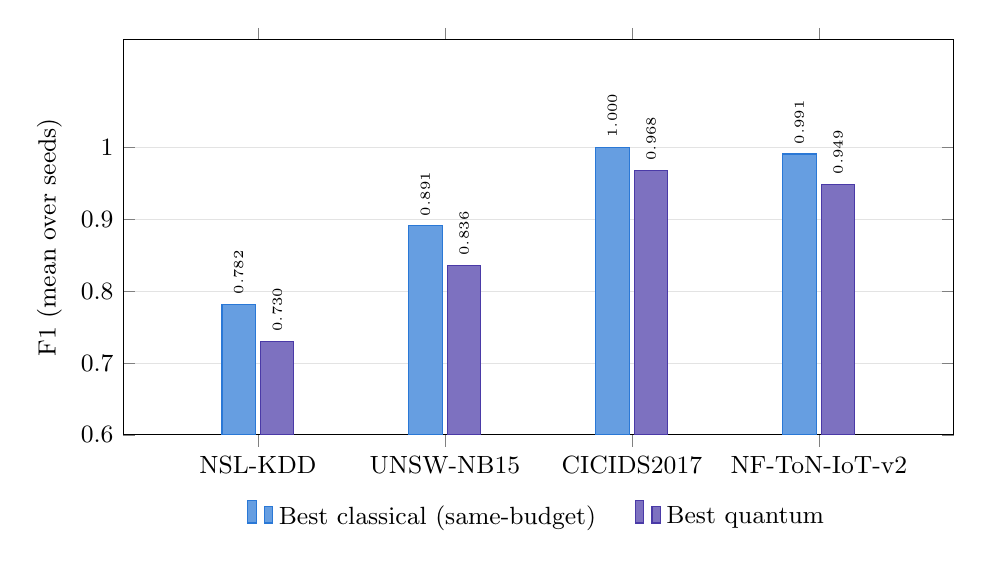
\begin{tikzpicture}
\begin{axis}[
  ybar, bar width=12pt,
  width=\textwidth, height=6.6cm,
  enlarge x limits=0.24,%
  ymin=0.6, ymax=1.15,%
  ytick={0.6,0.7,0.8,0.9,1.0},
  ylabel={F1 (mean over seeds)},
  ylabel style={font=\small},
  y tick label style={font=\small},
  symbolic x coords={NSL-KDD,UNSW-NB15,CICIDS2017,NF-ToN-IoT-v2},
  xtick=data,
  x tick label style={font=\small},
  legend style={at={(0.5,-0.15)},anchor=north,legend columns=2,font=\small,draw=none,
    /tikz/every even column/.append style={column sep=12pt}},
  nodes near coords,
  every node near coord/.append style={font=\tiny,rotate=90,anchor=west,
    /pgf/number format/.cd,fixed,fixed zerofill,precision=3},
  ymajorgrids,grid style={gray!22},
]
\addplot[fill=cvblue!72,draw=cvblue] coordinates
  {(NSL-KDD,0.782)(UNSW-NB15,0.891)(CICIDS2017,1.000)(NF-ToN-IoT-v2,0.991)};
\addplot[fill=cvviolet!72,draw=cvviolet] coordinates
  {(NSL-KDD,0.730)(UNSW-NB15,0.836)(CICIDS2017,0.968)(NF-ToN-IoT-v2,0.949)};
\legend{Best classical (same-budget),Best quantum}
\end{axis}
\end{tikzpicture}
\caption{Best classical (same-budget) vs.\ best quantum F1 per dataset (mean over seeds). Tuned
classical models lead on every dataset; the gap is largest on the discriminative datasets (NSL-KDD,
UNSW-NB15) and smallest where the task is near-saturated (CICIDS2017, NF-ToN-IoT-v2, where every
classical model exceeds $0.97$). The vertical axis is truncated at $0.6$.}
\label{fig:bars}
\end{figure}

\begin{figure}[t]
\centering
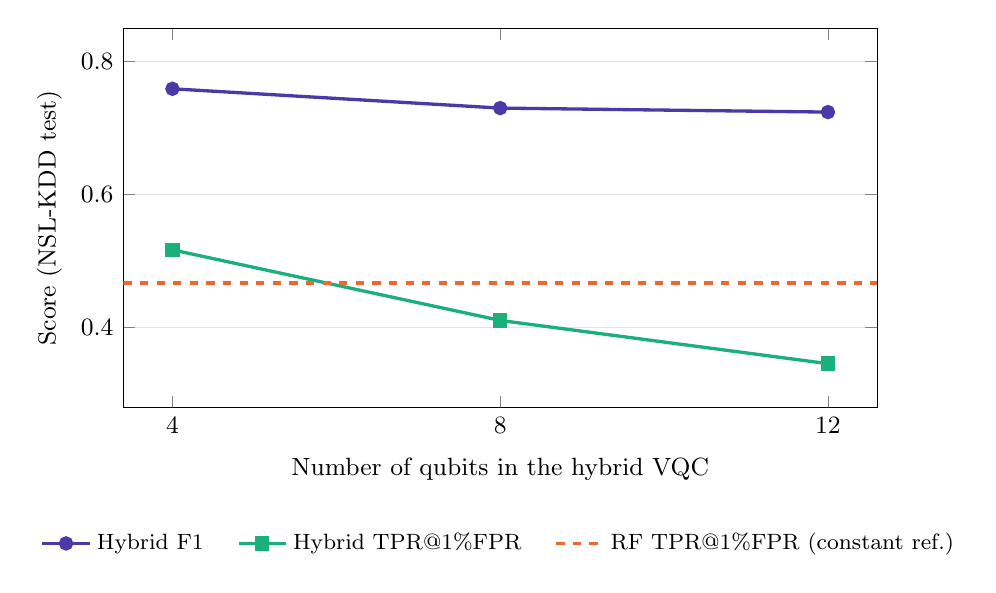
\begin{tikzpicture}
\begin{axis}[
  width=0.92\textwidth, height=6.4cm,
  xlabel={Number of qubits in the hybrid VQC},
  xlabel style={font=\small,yshift=-2pt},
  ylabel={Score (NSL-KDD test)},
  ylabel style={font=\small},
  tick label style={font=\small},
  xtick={4,8,12}, xmin=3.4, xmax=12.6,
  ymin=0.28, ymax=0.85,
  legend style={at={(0.5,-0.30)},anchor=north,legend columns=3,font=\footnotesize,draw=none,
    /tikz/every even column/.append style={column sep=10pt}},
  ymajorgrids,grid style={gray!22},
  every axis plot/.append style={very thick},
]
\addplot[cvviolet,mark=*] coordinates {(4,0.759)(8,0.730)(12,0.724)};
\addplot[cvaqua,mark=square*] coordinates {(4,0.517)(8,0.411)(12,0.346)};
\addplot[cvorange,dashed,mark=none] coordinates {(3.4,0.467)(12.6,0.467)};
\legend{Hybrid F1,Hybrid $\tpr$@$1\%\fpr$,RF $\tpr$@$1\%\fpr$ (constant ref.)}
\end{axis}
\end{tikzpicture}
\caption{Qubit-count ablation of the hybrid VQC on NSL-KDD. Both F1 and the low-FPR detection rate
\emph{decline} with width, so more qubits do not help on the shifted task. Crucially, only the small
four-qubit circuit exceeds the best classical baseline's $\tpr$@$1\%\fpr$ (Random Forest, dashed
reference at $0.467$); the advantage vanishes by twelve qubits, consistent with an
implicit-regularisation mechanism rather than raw expressivity.}
\label{fig:ablation}
\end{figure}

\section{Kernel-Level Analysis: How Quantum Is the Kernel Advantage?}\label{sec:kernel}
The audit's most robust positive was the quantum-kernel SVM out-ranking its random-feature surrogate
(Section~\ref{sec:audit-results}), the one comparison to survive both FDR and family-wise Holm
correction. That control, however, differed from the QSVM in four ways besides the feature map: it was
trained on 1{,}200 rather than 2{,}000 rows, it approximated its kernel with 512 Nystr\"om components,
it used a linear rather than a kernel SVM, and its bandwidth $\gamma=1$ was applied untuned to raw
features on a different scale. This section removes each difference in turn, examines how the result
depends on hyperparameter selection, tests it on a second official split, and asks whether what remains
requires the quantum state, and finally runs the kernel on real devices. The diagnostics are those of
Section~\ref{sec:kdiag}.

\subsection{The surrogate gap is set by the classical bandwidth search}\label{sec:kgap}
Table~\ref{tab:fair} places every kernel on the identical 2{,}000 NSL-KDD training rows, with exact Gram
matrices and one kernel SVM solver. Removing the first three confounds, with the bandwidth still fixed at
$\gamma=1$, narrows the published ROC-AUC gap from $0.127$ to $0.085$. Hyperparameter selection then
decides the outcome. With the bandwidth searched over $\gamma\le3$, cross-validation picks $\gamma=0.3$ for
the raw-feature RBF kernel, whose test ROC-AUC falls to $0.783$: an apparent quantum advantage of $0.167$
(95\% CI $[0.161,0.173]$). With the same cross-validation over $\gamma\le30$ it picks $\gamma=30$, and the RBF
kernel reaches $0.940$. The quantum kernel then leads by only $0.007$ in ROC-AUC ($[0.006,0.009]$) and
\emph{trails} at the operating point, where the classical kernel detects $0.455$ of attacks at $1\%$ false
positives against $0.442$ ($\Delta=-0.013$, $[-0.020,-0.005]$, $p=0.002$). The advantage the audit reported
is therefore not a property of the kernels. It appears or disappears with the width of the classical
baseline's search grid, a special case of the bandwidth sensitivity documented for quantum kernels by
Shaydulin and Wild~\cite{shaydulin2022bandwidth}, here acting on the \emph{classical} side of the
comparison. Schnabel and Roth~\cite{schnabel2025scrutiny} likewise find bandwidth and regularisation to
dominate quantum-kernel performance; what is new here is that a distribution shift makes the classical
baseline's choice of them unobservable to cross-validation.

\begin{table}[t]
\centering
\caption{Kernels on identical data (first 2{,}000 NSL-KDD training rows; official test set of
22{,}544 rows containing 17 attack types absent from training). Exact Gram matrices and one kernel SVM
solver throughout. \emph{Score} is the selection criterion's own value: in-distribution 5-fold CV AUC,
or leave-attack-types-out CV AUC for shift-aware rows. The phase kernel is an RBF kernel on
$(\sin x_i,\cos x_i)$ plus the ZZ feature map's phases, with no quantum state. Fixed rows use
$\gamma=1$, $C=1$. Generated from the result files.}
\label{tab:fair}
\scriptsize
\renewcommand{\arraystretch}{1.12}
\setlength{\tabcolsep}{3pt}
\begin{tabularx}{\textwidth}{@{}Ylccccc@{}}
\toprule
\textbf{Kernel} & \textbf{Feat.} & \textbf{Selection} & \textbf{Score} & \textbf{Test AUC} & \textbf{AUPRC} & \textbf{TPR@1\%FPR}\\
\midrule
\multicolumn{7}{@{}l}{\emph{Quantum}}\\
IQP projected, published & 24 & fixed & n/a & 0.945 & 0.957 & 0.470\\
IQP projected & 24 & CV, $\gamma\le3$ & 0.993 & 0.950 & 0.959 & 0.444\\
IQP projected & 24 & CV, $\gamma\le30$ & 0.994 & 0.948 & 0.957 & 0.442\\
IQP projected & 24 & shift-aware CV & 0.941 & 0.945 & 0.962 & 0.499\\
IQP fidelity & 256 & CV, $C$ only & 0.992 & 0.947 & 0.955 & 0.458\\
\addlinespace[2pt]
\multicolumn{7}{@{}l}{\emph{Classical, no quantum state}}\\
Random features, 1{,}200 rows, published & 512 & fixed & n/a & 0.818 & 0.885 & 0.352\\
Random features, 2{,}000 rows & 512 & fixed & n/a & 0.830 & 0.878 & 0.053\\
RBF, raw features & 8 & fixed & n/a & 0.861 & 0.892 & 0.045\\
RBF, raw features & 8 & CV, $\gamma\le3$ & 0.993 & 0.783 & 0.864 & 0.078\\
RBF, raw features & 8 & CV, $\gamma\le30$ & 0.994 & 0.940 & 0.953 & 0.455\\
RBF, raw features & 8 & shift-aware CV & 0.948 & 0.939 & 0.951 & 0.466\\
Trig $(\sin x_i,\cos x_i)$ only & 16 & CV, $\gamma\le3$ & 0.993 & 0.811 & 0.878 & 0.077\\
Phase kernel & 46 & CV, $\gamma\le3$ & 0.995 & 0.941 & 0.952 & 0.446\\
Phase kernel & 46 & CV, $\gamma\le30$ & 0.995 & 0.938 & 0.946 & 0.441\\
Phase kernel & 46 & shift-aware CV & 0.951 & 0.947 & 0.959 & 0.469\\
\bottomrule
\end{tabularx}
\end{table}

\subsection{Cross-validation cannot see the novel-attack shift}\label{sec:kcv}
Figure~\ref{fig:landscape} shows why the grid matters so much. Within the training distribution every
kernel scores between $0.95$ and $0.99$ at every bandwidth for $C=1$, so the cross-validation surface is nearly flat
and its maximum is close to arbitrary. On the official test set, whose 17 attack types never occur in
training, the raw-feature RBF kernel is U-shaped in $\gamma$: strong at very wide and very narrow
bandwidths (up to $0.945$), and weakest at intermediate ones ($0.740$ at worst across the grid), which is exactly where a
grid capped at $\gamma=3$ leads cross-validation. Across the 40 settings of the grid the RBF kernel's
standard CV score is uncorrelated with its test ROC-AUC ($r=-0.16$).

This motivates \emph{shift-aware model selection}: leave-attack-types-out cross-validation, in which each
attack type lives in exactly one fold, so every validation fold contains attack types its training fold
never saw. It reproduces the condition of the official split using training data alone; attack types
are assigned to folds by GroupKFold, and the three of five folds in which both classes occur are used.
Its score correlates with test ROC-AUC at $r=+0.79$ for the RBF kernel, and it selects robust settings for every
kernel family, with test ROC-AUC between $0.939$ and $0.947$ (Table~\ref{tab:fair}). Under this rule the
quantum projected kernel also reaches the highest operating-point detection we observe,
$\tpr$@$1\%\fpr=0.499$, above the RBF kernel's $0.466$ ($\Delta=+0.033$, $[0.021,0.067]$, $p<0.001$). We do
not read this as a quantum advantage, because its sign depends on the selection rule: under standard CV
the same comparison favours the classical kernel by $0.013$. Having now evaluated three selection rules,
reporting only the one on which quantum wins would be precisely the researcher degree of freedom this
paper warns against.

\begin{figure}[t]
\centering
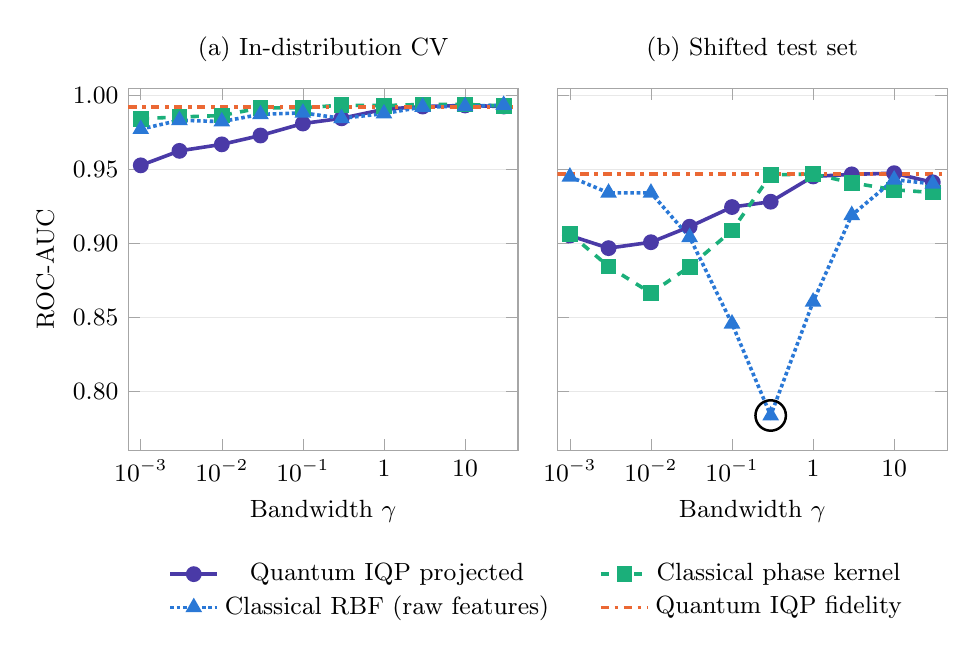
\begin{tikzpicture}
\begin{groupplot}[
  group style={group size=2 by 1, horizontal sep=0.5cm, y descriptions at=edge left},
  scale only axis, width=4.95cm, height=4.6cm,
  xmode=log, xmin=0.0007, xmax=45,
  xminorticks=false,
  ymin=0.76, ymax=1.005,
  xtick={0.001,0.01,0.1,1,10},
  xticklabels={$10^{-3}$,$10^{-2}$,$10^{-1}$,$1$,$10$},
  ytick={0.8,0.85,0.9,0.95,1.0},
  yticklabel style={/pgf/number format/.cd,fixed,fixed zerofill,precision=2},
  xlabel={Bandwidth $\gamma$},
  tick label style={font=\small}, label style={font=\small}, title style={font=\small},
  ymajorgrids, grid style={gray!18},
  axis line style={gray!70}, tick style={gray!70},
  every axis plot/.append style={line width=1.3pt, mark size=2.2pt},
]
\nextgroupplot[title={(a) In-distribution CV}, ylabel={ROC-AUC}]
\addplot[cvviolet, mark=*] coordinates
  {(0.001,0.9528)(0.003,0.9626)(0.01,0.9670)(0.03,0.9730)(0.1,0.9811)(0.3,0.9846)(1,0.9907)(3,0.9926)(10,0.9933)(30,0.9926)};
\addplot[cvaqua, dashed, mark=square*, mark options={solid}] coordinates
  {(0.001,0.9844)(0.003,0.9855)(0.01,0.9865)(0.03,0.9917)(0.1,0.9917)(0.3,0.9935)(1,0.9932)(3,0.9940)(10,0.9940)(30,0.9930)};
\addplot[cvblue, densely dotted, mark=triangle*, mark options={solid}] coordinates
  {(0.001,0.9773)(0.003,0.9833)(0.01,0.9824)(0.03,0.9873)(0.1,0.9883)(0.3,0.9846)(1,0.9878)(3,0.9923)(10,0.9927)(30,0.9936)};
\addplot[cvorange, dash dot, mark=none] coordinates {(0.0007,0.9924)(45,0.9924)};

\nextgroupplot[title={(b) Shifted test set},
  legend style={at={(-0.05,-0.28)}, anchor=north, legend columns=2, draw=none,
    font=\small, /tikz/every even column/.append style={column sep=16pt}}]
\addplot[cvviolet, mark=*] coordinates
  {(0.001,0.9053)(0.003,0.8968)(0.01,0.9008)(0.03,0.9113)(0.1,0.9246)(0.3,0.9282)(1,0.9453)(3,0.9467)(10,0.9475)(30,0.9413)};
\addplot[cvaqua, dashed, mark=square*, mark options={solid}] coordinates
  {(0.001,0.9066)(0.003,0.8844)(0.01,0.8664)(0.03,0.8843)(0.1,0.9087)(0.3,0.9463)(1,0.9470)(3,0.9410)(10,0.9363)(30,0.9344)};
\addplot[cvblue, densely dotted, mark=triangle*, mark options={solid}] coordinates
  {(0.001,0.9451)(0.003,0.9342)(0.01,0.9342)(0.03,0.9042)(0.1,0.8457)(0.3,0.7836)(1,0.8605)(3,0.9191)(10,0.9431)(30,0.9403)};
\addplot[cvorange, dash dot, mark=none] coordinates {(0.0007,0.9471)(45,0.9471)};
\draw[black, line width=0.9pt] (axis cs:0.3,0.7836) circle (5.5pt);
\legend{Quantum IQP projected, Classical phase kernel,
        Classical RBF (raw features), Quantum IQP fidelity}
\end{groupplot}
\end{tikzpicture}
\caption{Kernel performance across the RBF bandwidth on NSL-KDD ($C=1$, first 2{,}000 training rows).
(a) Within the training distribution every kernel scores $0.95$ to $0.99$ at every bandwidth, so
cross-validation cannot tell good settings from bad ones. (b) On the official test set, whose 17
attack types never occur in training, the raw-feature RBF kernel collapses at intermediate bandwidths
while recovering at both extremes. Standard CV over a grid capped at $\gamma=3$ selects $\gamma=0.3$
($C=100$), test ROC-AUC $0.783$, at the circled dip; with the grid extended to $\gamma=30$ it selects
$\gamma=30$ ($C=1$), test ROC-AUC $0.940$. The classical phase kernel uses the ZZ feature map's phases with
no quantum state; the IQP fidelity kernel has no bandwidth and is drawn as a constant. On this dataset the
quantum projected kernel never falls below $0.893$ across the full grid, against $0.740$ for the
raw-feature RBF; on UNSW-NB15 the order reverses (Section~\ref{sec:kunsw}).}
\label{fig:landscape}
\end{figure}

\subsection{A second official split}\label{sec:kunsw}
If the collapse of standard CV is caused by novel attack types, it should vanish on a dataset whose test
set has none. UNSW-NB15 is the only other benchmark here with an official split, and every one of its
nine attack categories occurs in both training and test. We repeat the protocol on a seeded, stratified
sample of 2{,}000 training rows and 20{,}000 test rows; the training file is sorted by class, so its first
rows are all benign and cannot be used. Table~\ref{tab:twosplits} confirms the prediction: on UNSW-NB15
standard CV tracks test performance for every kernel ($r=+0.82$ to $+0.83$). The result for the quantum
kernel, however, reverses. Selected by the same rule, it is significantly worse than both classical kernels
on every metric: the classical phase kernel of Section~\ref{sec:kgeom} reaches test ROC-AUC $0.956$ against
$0.930$ ($\Delta=-0.026$, $[-0.028,-0.024]$) and detects $0.751$ of attacks at $1\%$ false positives against
$0.457$ ($\Delta=-0.294$, $[-0.318,-0.263]$), and even the raw-feature RBF kernel is ahead ($\Delta\tpr=-0.057$,
$[-0.087,-0.022]$, $p=0.005$). The one property that had favoured the quantum kernel on NSL-KDD, fewer poor
hyperparameter settings (worst test ROC-AUC $0.893$ against $0.740$), does not survive either: on
UNSW-NB15 its worst setting is the lowest of the three ($0.697$ against $0.787$ and $0.789$). We therefore do
not claim it as a property of quantum kernels. Shift-aware CV on UNSW-NB15, whose official split has no
novel attacks for it to anticipate, is examined with the induced-shift experiment in
Section~\ref{sec:kinduced}.

\begin{table}[t]
\centering
\caption{Kernels on the two datasets with an official train/test split, each selected by standard
5-fold CV over the full grid ($\gamma\le30$, $C\le100$). \emph{Worst} is the lowest test ROC-AUC over all
40 settings; $r$ is the correlation, across those settings, between the CV score and the test ROC-AUC.
NSL-KDD's test set contains 17 attack types absent from training; UNSW-NB15's contains none. Generated
from the result files.}
\label{tab:twosplits}
\scriptsize
\renewcommand{\arraystretch}{1.15}
\setlength{\tabcolsep}{4pt}
\begin{tabularx}{\textwidth}{@{}lYccccc@{}}
\toprule
\textbf{Dataset} & \textbf{Kernel} & \textbf{Test AUC} & \textbf{AUPRC} & \textbf{TPR@1\%FPR} & \textbf{Worst} & $\bm{r}$\\
\midrule
\multirow{3}{*}{NSL-KDD} & Quantum IQP projected & 0.948 & 0.957 & 0.442 & 0.893 & $+0.83$\\
 & Phase kernel (classical) & 0.938 & 0.946 & 0.441 & 0.818 & $+0.24$\\
 & RBF, raw features (classical) & 0.940 & 0.953 & 0.455 & 0.740 & $-0.16$\\
\addlinespace[3pt]
\multirow{3}{*}{UNSW-NB15} & Quantum IQP projected & 0.930 & 0.943 & 0.457 & 0.697 & $+0.82$\\
 & Phase kernel (classical) & 0.956 & 0.968 & 0.751 & 0.787 & $+0.83$\\
 & RBF, raw features (classical) & 0.938 & 0.951 & 0.514 & 0.789 & $+0.83$\\
\bottomrule
\end{tabularx}
\end{table}

\subsection{Inducing the shift}\label{sec:kinduced}
The contrast between the two datasets is consistent with the novel-attack explanation but does not test
it, because the datasets differ in more than their splits. We therefore induce the shift on UNSW-NB15
itself: whole attack categories are removed from the 2{,}000-row training sample and left in the
20{,}000-row test sample, and the protocol of Table~\ref{tab:twosplits} is repeated. Two holdouts guard
against a lucky choice. Holdout A removes Exploits, Fuzzers and Reconnaissance, which then make up $25\%$
of the test rows; holdout B removes Generic, DoS, Analysis and Backdoor, $29\%$ of the test rows.
Table~\ref{tab:induced} gives the result.

Unseen attack types are necessary for the failure but not sufficient. Under holdout A standard CV still
ranks the grid correctly for every kernel ($r=+0.85$ to $+0.99$) and its choices lie within $0.009$
ROC-AUC of the best setting in the grid. Under holdout B the NSL-KDD picture returns. Every kernel loses
between $0.06$ and $0.16$ ROC-AUC at its best setting, the correlation between CV score and test ROC-AUC
falls to $+0.62$ to $+0.69$, and the loss from selection is unequal across kernels: the CV-selected
raw-feature RBF kernel sits $0.108$ below its oracle ($0.794$ against $0.902$), the quantum kernel
$0.028$ below ($0.761$ against $0.789$). A comparison made at the CV-selected settings therefore
understates the classical kernel's lead by $0.08$ ROC-AUC, and at $1\%$ false positives it reverses the
order outright: the quantum kernel detects $0.302$ of attacks against $0.263$ for the RBF kernel, whose
best setting in the grid detects $0.465$. This is the mechanism of Section~\ref{sec:kcv} reproduced on
demand, on a dataset on which it was absent, by changing nothing but which attack types the training
sample contains. What separates the two holdouts is the bandwidth landscape: under holdout B the RBF
kernel's test ROC-AUC peaks sharply at $\gamma=0.3$ ($0.902$, against $0.794$ at $\gamma=0.1$ and
$0.864$ at $\gamma=1$) while its CV score is flat across those settings ($0.966$ to $0.967$), so the
selection criterion cannot resolve the one setting that generalises to the unseen categories.

Shift-aware selection does not repair holdout B. Leave-attack-types-out CV, which restored selection on
NSL-KDD, correlates with test ROC-AUC at $r=+0.43$ for the RBF kernel here and chooses a setting worse
than standard CV ($0.751$). Its folds can only hold out attack types the training sample contains
(Exploits, Fuzzers, Reconnaissance, Shellcode, Worms), and a shift towards those types is not the shift
towards Generic and DoS that the test set presents. On NSL-KDD the seventeen unseen types are variants
within the same four attack families as the seen ones, which is why holding out types reproduces the
official split there. Nor is the result an artefact of how the folds are built. The construction used
throughout assigns attack types to folds with GroupKFold, which leaves three usable folds on NSL-KDD and
one on UNSW-NB15; an alternative that splits the benign rows evenly and assigns attack types largest-first
to the emptiest fold makes all five folds usable on every dataset, but gives $r=+0.54$ instead of $+0.79$
for the RBF kernel on NSL-KDD, $r=-0.38$ under holdout B, and on the official UNSW-NB15 split, which has
no unseen types, it selects an over-smooth bandwidth for the RBF kernel (test ROC-AUC $0.859$ against
$0.938$ under standard CV). Shift-aware selection is a choice of target rather than a free improvement:
it buys robustness to the kinds of novelty the training data can imitate, at a cost when there is no
novelty to be robust to, and it cannot anticipate novelty of a kind the training data has never seen.
The general lesson is procedural. A kernel comparison under distribution shift should be reported under
more than one selection rule, with the oracle bound alongside, so that a reader can see how much of a
claimed difference is selection.

\begin{table}[!htb]
\centering
\caption{Inducing novel-attack shift on UNSW-NB15. Whole attack categories are removed from the
2{,}000-row training sample and kept in the 20{,}000-row test sample: holdout A removes Exploits, Fuzzers, Recon. (25\% of test rows); holdout B removes Generic, DoS, Analysis, Backdoor (29\% of test rows). Each kernel is
selected by standard 5-fold CV over the full grid ($\gamma\le30$, $C\le100$); $r$ is the correlation
across the 40 settings between the CV score and the test ROC-AUC, and \emph{oracle} the best test ROC-AUC
in the grid. The last two columns give TPR@1\%FPR at the CV-selected setting and the best in the grid.
Generated from the result files.}
\label{tab:induced}
\scriptsize
\renewcommand{\arraystretch}{1.15}
\setlength{\tabcolsep}{3pt}
\begin{tabularx}{\textwidth}{@{}lYccccc@{}}
\toprule
& & & \multicolumn{2}{c}{\textbf{Test ROC-AUC}} & \multicolumn{2}{c}{\textbf{TPR@1\%FPR}}\\
\cmidrule(lr){4-5}\cmidrule(lr){6-7}
\textbf{Unseen types} & \textbf{Kernel} & $\bm{r}$ & \textbf{CV pick} & \textbf{Oracle} & \textbf{CV pick} & \textbf{Best}\\
\midrule
\multirow{3}{*}{None (0\%)} & Quantum IQP projected & $+0.82$ & 0.930 & 0.948 & 0.457 & 0.561\\
 & Phase kernel (classical) & $+0.83$ & 0.956 & 0.957 & 0.751 & 0.751\\
 & RBF, raw features (classical) & $+0.83$ & 0.938 & 0.957 & 0.514 & 0.661\\
\addlinespace[3pt]
\multirow{3}{*}{Holdout A (25\%)} & Quantum IQP projected & $+0.99$ & 0.936 & 0.940 & 0.739 & 0.744\\
 & Phase kernel (classical) & $+0.85$ & 0.938 & 0.947 & 0.714 & 0.764\\
 & RBF, raw features (classical) & $+0.92$ & 0.940 & 0.946 & 0.708 & 0.779\\
\addlinespace[3pt]
\multirow{3}{*}{Holdout B (29\%)} & Quantum IQP projected & $+0.69$ & 0.761 & 0.789 & 0.302 & 0.344\\
 & Phase kernel (classical) & $+0.62$ & 0.844 & 0.861 & 0.413 & 0.487\\
 & RBF, raw features (classical) & $+0.69$ & 0.794 & 0.902 & 0.263 & 0.465\\
\bottomrule
\end{tabularx}
\end{table}

\subsection{Geometry: the IQP kernel is close to its own classical phases}\label{sec:kgeom}
Table~\ref{tab:geom} gives the geometric difference on all four datasets, which requires no labels and no
hyperparameter selection. The angle-encoded fidelity kernel is reproduced by an RBF kernel to $g=1.06$ to
$1.07$ on every dataset, so by the bound of Huang et al.~\cite{huang2021power} it can hold no prediction
advantage over that classical kernel for any labelling. This is expected: under angle encoding every qubit
remains in a product state, and the kernel factorises into a product of cosines. The IQP kernels, which
use entangling ZZ gates, are genuinely far from standard kernels: against every RBF bandwidth and against
plain trigonometric features, $g$ ranges from $4.9$ to $12.2$. Fl\'orez-Ablan et al.~\cite{florezablan2025similarity}
show that optimally rescaling the encoding drives quantum kernels towards RBF kernels; our IQP kernels use
the unscaled encoding of the original pipeline, and consistently with that result they sit far from RBF. The same IQP kernels, however, lie within
$g=1.4$ to $2.4$ of a purely classical kernel built on the phases the ZZ feature map
writes~\cite{havlicek2019supervised}, on all four datasets, and their label-dependent model complexities
agree: on NSL-KDD the quantum projected kernel has $s_K=235$ and the classical phase kernel $s_K=236$, against
$481$ for the best raw-feature RBF. The empirical results are consistent with this geometry. On NSL-KDD the
phase kernel matches the quantum kernel at the operating point under a narrow grid ($0.446$ against
$0.444$, $p=0.89$) and under standard CV over the full grid ($0.441$ against $0.442$, $p=0.90$), and on
UNSW-NB15 it outperforms it. Whatever the IQP kernel contributes lives in the phases of its circuit, not
in the quantum state, and a classical kernel that uses those phases obtains it at a small fraction of the
cost.

\begin{table}[t]
\centering
\caption{Geometric difference $g(K_C\Vert K_Q)$, minimised over classical bandwidth
($N=800$, $\lambda=10^{-2}$, $\sqrt{N}\approx 28.3$). A small $g$ means the
classical kernel can learn anything the quantum kernel can. The last column gives the angle-encoded
fidelity kernel against its best RBF. Rank-deficient kernels are excluded. Generated from the result
files.}
\label{tab:geom}
\footnotesize
\renewcommand{\arraystretch}{1.15}
\setlength{\tabcolsep}{3pt}
\begin{tabular}{@{}llcccc@{}}
\toprule
& & \multicolumn{3}{c}{\textbf{Classical family, vs IQP kernel}} & \textbf{Angle fidelity}\\
\cmidrule(lr){3-5}\cmidrule(lr){6-6}
\textbf{Dataset} & \textbf{IQP kernel} & \textbf{RBF raw} & \textbf{Trig} & \textbf{Phase kernel} & \textbf{vs RBF}\\
\midrule
NSL-KDD & projected & 8.41 & 8.33 & \textbf{2.27} & \multirow{2}{*}{1.07}\\
 & fidelity & 4.91 & 4.88 & \textbf{1.77} & \\
UNSW-NB15 & projected & 12.21 & 12.10 & \textbf{2.44} & \multirow{2}{*}{1.07}\\
 & fidelity & 9.52 & 9.34 & \textbf{1.50} & \\
CICIDS2017 & projected & 8.65 & 8.48 & \textbf{1.95} & \multirow{2}{*}{1.06}\\
 & fidelity & 7.04 & 6.86 & \textbf{1.54} & \\
NF-ToN-IoT-v2 & projected & 9.25 & 9.07 & \textbf{2.23} & \multirow{2}{*}{1.07}\\
 & fidelity & 7.84 & 7.64 & \textbf{1.39} & \\
\bottomrule
\end{tabular}
\end{table}

\subsection{Concentration and finite shots}\label{sec:kshots}
Kernel values concentrate as width grows, but mildly at these sizes. From 2 to 12 qubits the mean
off-diagonal IQP fidelity falls from $0.32$ to $0.047$, yet its variance falls only from $0.099$ to $0.032$
and flattens between 8 and 10 qubits, far from the exponential regime of Thanasilp
et al.~\cite{thanasilp2024concentration}. The kernels' test ROC-AUC peaks at 8 to 10 qubits ($0.944$ to
$0.946$ for the projected kernel) and dips only to $0.927$ at 12. Concentration therefore does not explain
the decline of the variational hybrid with width (Figure~\ref{fig:ablation}), which points instead to the
trainability and capacity of the variational model.

The projected kernel is robust to measurement noise (Table~\ref{tab:shots}). With 16 shots in each of three
measurement bases, 48 shots per sample in total, test ROC-AUC falls from $0.945$ to $0.941$, and AUPRC and
$\tpr$@$1\%\fpr$ do not move beyond their run-to-run spread; by 64 shots the result is indistinguishable
from the exact kernel. This follows from the construction: the projected kernel needs only single-qubit
expectations, each estimated with variance at most $1/M$, which the RBF then smooths, whereas a fidelity
kernel must resolve small global overlaps. The study models sampling noise only; Section~\ref{sec:khw}
tests the same kernel, with its gate and readout errors, on real devices.

\begin{table}[t]
\centering
\caption{Finite-shot robustness of the published IQP projected QSVM on NSL-KDD. $M$ shots per basis in
each of the X, Y and Z settings; mean and standard deviation over 5 sampling seeds. Generated from the
result files.}
\label{tab:shots}
\footnotesize
\renewcommand{\arraystretch}{1.15}
\setlength{\tabcolsep}{6pt}
\begin{tabular}{@{}rrccc@{}}
\toprule
\textbf{Shots / basis} & \textbf{Shots / sample} & \textbf{ROC-AUC} & \textbf{AUPRC} & \textbf{TPR@1\%FPR}\\
\midrule
16 & 48 & $0.941\pm0.002$ & $0.956\pm0.002$ & $0.486\pm0.011$\\
64 & 192 & $0.945\pm0.002$ & $0.960\pm0.001$ & $0.489\pm0.009$\\
256 & 768 & $0.943\pm0.004$ & $0.957\pm0.002$ & $0.473\pm0.003$\\
1{,}024 & 3{,}072 & $0.943\pm0.002$ & $0.956\pm0.001$ & $0.469\pm0.002$\\
4{,}096 & 12{,}288 & $0.947\pm0.001$ & $0.957\pm0.001$ & $0.470\pm0.001$\\
\addlinespace[2pt]
exact & $\infty$ & $0.945$ & $0.957$ & $0.470$\\
\bottomrule
\end{tabular}
\end{table}

\subsection{On real hardware}\label{sec:khw}
Table~\ref{tab:hardware} reports the projected kernel executed on three IBM Heron processors,
\texttt{ibm\_fez}, \texttt{ibm\_kingston} and \texttt{ibm\_marrakesh}, on the same 200 training and 500
test samples, each as a single job of 89 to 91 QPU-seconds (Section~\ref{sec:kdiag}). The measured Pauli
features correlate with their exact values at $r=0.92$ to $0.97$ (RMSE $0.10$ to $0.15$), and the Gram
matrices built from them at $r=0.97$ to $0.98$; on \texttt{ibm\_fez} the Gram correlation of $0.977$
matches the $r\ge0.976$ that Kakavand et al.~\cite{kakavand2026benchmarking} report for the same device.
The classifier trained and tested on measured features alone reaches ROC-AUC $0.935$, $0.935$ and $0.942$
against $0.944$ for the exact kernel: a deficit of $0.009$ on \texttt{ibm\_fez} (95\% CI $[0.000,0.018]$,
$p=0.049$) and on \texttt{ibm\_kingston} ($[0.002,0.018]$, $p=0.017$), and none on \texttt{ibm\_marrakesh}
($[-0.002,0.007]$, $p=0.35$). AUPRC shows a significant deficit only on \texttt{ibm\_kingston} ($0.011$,
$p=0.002$), and at the $1\%$ false-positive operating point no device differs from the exact kernel
(measured $0.404$ to $0.408$ against $0.396$, $p\ge0.62$). The mechanism anticipated in
Section~\ref{sec:kshots} holds on hardware: per-feature noise well above the shot-noise floor is largely
absorbed by the RBF over 24 features.

Two caveats apply. The devices were noisier at the feature level than the calibration-based noise model
of the dry run predicted (test RMSE $0.15$ on \texttt{ibm\_fez} against $0.07$ in simulation), so noise
models of this kind should not be taken as substitutes for device runs. And hardware validity is not
advantage: the same measured features are, by Section~\ref{sec:kgeom}, reproducible by a classical kernel
on the circuit's phases. What the device runs establish is that the object we analysed is realisable at
current noise levels, at a cost of about $0.13$ QPU-seconds per sample.

\begin{table}[t]
\centering
\caption{Hardware validation of the IQP projected kernel on NSL-KDD (200 training and
500 test samples, the latter class-balanced). Agreement columns are Pearson correlations
of the source's Pauli features and of its Gram matrix (off-diagonal) with the exact statevector values.
Metric columns are for the projected-kernel SVM trained and tested on that source's own features
($\gamma=1$, $C=1$). Generated from the result files.}
\label{tab:hardware}
\footnotesize
\renewcommand{\arraystretch}{1.15}
\setlength{\tabcolsep}{3pt}
\begin{tabularx}{\textwidth}{@{}Yccccc@{}}
\toprule
& \multicolumn{2}{c}{\textbf{Agreement with exact}} & \multicolumn{3}{c}{\textbf{Projected-kernel SVM}}\\
\cmidrule(lr){2-3}\cmidrule(lr){4-6}
\textbf{Feature source} & \textbf{Feat.\ $r$} & \textbf{Gram $r$} & \textbf{ROC-AUC} & \textbf{AUPRC} & \textbf{TPR@1\%FPR}\\
\midrule
Exact statevector & 1.000 & 1.000 & 0.944 & 0.941 & 0.396\\
Noisy simulation (FakeFez, 256 shots) & 0.984 & 0.990 & 0.941 & 0.938 & 0.420\\
\texttt{ibm\_fez} (128 shots) & 0.920 & 0.977 & 0.935 & 0.935 & 0.404\\
\texttt{ibm\_kingston} (128 shots) & 0.941 & 0.971 & 0.935 & 0.930 & 0.404\\
\texttt{ibm\_marrakesh} (128 shots) & 0.966 & 0.984 & 0.942 & 0.939 & 0.408\\
\bottomrule
\end{tabularx}
\end{table}

The device runs also settle the status of the audit's one surviving positive.
Section~\ref{sec:audit-results} left the four-qubit hybrid's advantage over the tuned Random Forest at
$1\%$ false positives as a hypothesis for hardware testing; Table~\ref{tab:hybridhw} tests it. On
2{,}000 class-balanced test rows the retrained model's exact scores give ROC-AUC $0.900$ and
$\tpr$@$1\%\fpr=0.496$, against $0.929$ and $0.304$ for the Random Forest on the same rows, so the pattern
of Table~\ref{tab:audit} is present in this sample: the forest is better on aggregate ($\Delta$ROC-AUC
$=-0.029$, $[-0.042,-0.017]$) and the hybrid better at the low-false-positive operating point
($\Delta\tpr=+0.192$, $[0.009,0.296]$, $p=0.031$). With the four expectations measured on
\texttt{ibm\_fez}, \texttt{ibm\_kingston} and \texttt{ibm\_marrakesh} instead of simulated, they
correlate with their exact values at $r=0.97$ to $0.98$ (RMSE $0.11$ to $0.12$, of which shot noise at
128 shots accounts for up to $0.09$), the final scores at $r=0.99$, and the model's ROC-AUC falls by
$0.017$ to $0.020$ on every device ($p<0.001$): close to the $0.012$ that shot noise alone costs in
simulation, with a device contribution below $0.01$. The operating-point result is untouched.
$\tpr$@$1\%\fpr$ is $0.498$, $0.498$ and $0.501$ on the three devices against $0.496$ exact ($p\ge0.9$),
and the margin over the Random Forest on the same rows is $+0.194$, $+0.194$ and $+0.197$ ($p=0.033$,
$0.058$ and $0.047$). The low-FPR result therefore survives real device noise on three processors, which
is more than the simulated audit could say. It remains what it was: a comparison between a variational
model and a tree ensemble on one dataset, resting here on 1{,}000 benign rows, and not an attribution to
the quantum layer, whose four-qubit circuit is well within classical reach. The cost was 86 to 87
QPU-seconds per device for 2{,}000 samples, about $0.04$ QPU-seconds per sample.

\begin{table}[!htb]
\centering
\caption{The 4-qubit hybrid on hardware: NSL-KDD, 2{,}000 class-balanced test rows.
Only the four $\langle Z_i\rangle$ that feed the trained classical head are measured; every other part of
the model is the published one. $r$ is the Pearson correlation of the source's expectations with the
exact statevector values. Metric columns are the hybrid's own on that source; the shot-noise row is the
mean of 20 binomial resamplings of the exact expectations. The last column is the
paired-bootstrap difference in TPR@1\%FPR against the tuned random forest on the same rows (positive
favours the hybrid; two-sided $p$ in brackets). Generated from the result files.}
\label{tab:hybridhw}
\scriptsize
\renewcommand{\arraystretch}{1.15}
\setlength{\tabcolsep}{3pt}
\begin{tabularx}{\textwidth}{@{}Yccccc@{}}
\toprule
& & \multicolumn{3}{c}{\textbf{Hybrid QNN}} & \\
\cmidrule(lr){3-5}
\textbf{Source of $\langle Z_i\rangle$} & $\bm{r}$ & \textbf{ROC-AUC} & \textbf{AUPRC} & \textbf{TPR@1\%FPR} & $\bm{\Delta}$\textbf{TPR vs RF}\\
\midrule
Exact statevector & 1.000 & 0.900 & 0.914 & 0.496 & $+0.192$ [$0.03$]\\
Shot noise only (128 shots) &  & 0.888 & 0.909 & 0.502 & \\
FakeFez simulation (128 shots) & 0.981 & 0.881 & 0.905 & 0.495 & \\
\texttt{ibm\_fez} (128 shots) & 0.976 & 0.883 & 0.906 & 0.498 & $+0.194$ [$0.03$]\\
\texttt{ibm\_kingston} (128 shots) & 0.972 & 0.882 & 0.904 & 0.498 & $+0.194$ [$0.06$]\\
\texttt{ibm\_marrakesh} (128 shots) & 0.976 & 0.880 & 0.904 & 0.501 & $+0.197$ [$0.05$]\\
\addlinespace[2pt]
Tuned random forest, same rows &  & 0.929 & 0.917 & 0.304 & \\
\bottomrule
\end{tabularx}
\end{table}

\subsection{Summary}\label{sec:ksum}
Once kernels are compared on identical data with equal and adequate tuning, no quantum-kernel advantage
survives the choice of selection rule or of dataset. The audit's strongest positive was produced by its
own classical surrogate: first by four confounds, then by a bandwidth grid too narrow for a distribution
shift that in-distribution cross-validation cannot see. Three findings of general use come out of the
exercise. The selection failure can be induced at will by holding attack families out of training, and
no training-only rule repairs it in general: leave-attack-types-out cross-validation restores selection
on NSL-KDD, where the unseen attacks are relatives of seen ones, but not under the induced shift, so
kernel comparisons under shift should be reported under several rules with the oracle bound. The
geometric difference identifies, without labels, when a quantum kernel is classically reproducible, which
here it is from its own circuit phases on every dataset. And the objects under analysis run on current
hardware: on three IBM Heron processors the projected kernel's measured Gram matrix correlates at $0.97$
to $0.98$ with simulation and its classifier stays within $0.01$ ROC-AUC of the exact kernel, and the
four-qubit hybrid keeps its low-false-positive margin over the Random Forest, so neither the classical
reproducibility nor the one surviving positive is an artefact of simulation.

\section{Discussion}

\textbf{How quantum is the advantage?} On this benchmark and in the practical NISQ regime, almost none of
it. The audit settles the aggregate question: once a classical model is granted the same front-end and
comparable regularisation, the aggregate advantage of the hybrid VQC and the QSVM vanishes, and tuned
classical baselines significantly outperform the quantum models on F1 and AUPRC. We thus confirm the
Bellante et al.~\cite{bellante2025pca} hypothesis and extend it from their fault-tolerant, PCA-specific
case study to the deployed NISQ models, and we corroborate Bhatnagar et al.'s
concession~\cite{bhatnagar2026mqe} while supplying the decomposition their work lacked.

The kernel-level analysis settles the exception we had expected to be the most robust. The quantum
kernel's advantage over its classical surrogate survived both FDR and family-wise correction, yet it was
not quantum: it came from four confounds in the surrogate and then from the width of the classical
bandwidth grid (Section~\ref{sec:kernel}). This is a cautionary result for the field, not only for this
paper. Statistical robustness does not establish attribution, and under the distribution shift that makes
NIDS evaluation meaningful, the classical baseline's hyperparameter search can manufacture or erase an
apparent quantum advantage. A QML-IDS claim evaluated on a split with unseen attack types should report
how its classical baselines were tuned, over what range, and by which selection rule, and should report
the comparison under more than one rule with the oracle bound, since no training-only rule, shift-aware
selection included, proved reliable under every shift we induced.

One narrower positive remains from the audit. At the $1\%$-$\fpr$ operating point on NSL-KDD the
four-qubit hybrid out-detects the tuned Random Forest ($p=0.005$, BH $q=0.030$), although it does not
survive the more conservative Holm correction. It appears on the discriminative dataset rather than the
saturated ones, and it is strongest for the small circuit and vanishes at twelve qubits, consistent with
implicit regularisation rather than expressivity. Our noise sweep used a six-qubit hybrid, so it does not
bear on this configuration. On three IBM Heron processors it reproduces with the quantum layer's
expectations measured rather than simulated (Section~\ref{sec:khw}), so it is not an artefact of
noiseless simulation; but it remains a comparison between a variational model and a tree ensemble on one
dataset, a comparison the kernel-level controls of Section~\ref{sec:kernel} do not address, and we do
not regard it as evidence of quantum advantage.

\textbf{What remains classical.} For a practitioner choosing a detector today, the honest recommendation
is a tuned Random Forest or XGBoost: they win or tie on every aggregate metric, on every dataset, at a
fraction of the cost and with no quantum hardware. Three methodological findings generalise. The
$\approx 0.20$ F1 CV-to-test gap is a caution for the whole QML-IDS literature; leave-attack-types-out
cross-validation addresses the model-selection failure behind it on NSL-KDD, and the induced-shift
experiment shows where such rules stop working; and the backend crossover (the GPU is an
order of magnitude \emph{slower} at these qubit counts) saves researchers real time.

\section{Limitations and Threats to Validity}
\textbf{Hardware.} The projected quantum kernel and the four-qubit hybrid's quantum layer were executed
on three IBM Heron processors (Section~\ref{sec:khw}); every other quantum result, including the wider
hybrids and the noise sweep, is simulated, and the noise sweep models NISQ effects rather than measuring
them. The device runs used 200 training and 500 test samples for the kernel and 2{,}000 test samples for
the hybrid, 128 shots per basis, and only the primitive's default readout mitigation; they realise
inference, not training, on hardware, and the fidelity kernel, whose cost is quadratic in the sample
count, was not run. The hybrid's low-false-positive margin on hardware rests on 1{,}000 benign rows, so
its $1\%$ threshold is set by ten scores and its confidence intervals are wide.
\textbf{Qubit budget.} The 4\,GB GPU caps width at roughly sixteen qubits (noiseless) / twelve (noisy,
$(2^n)^2$ memory); the main configuration uses eight, so we cannot probe the larger-width regime.
\textbf{Dimensionality reduction} discards variance (eight PCs retain $\sim$84\% on NSL-KDD), so any
advantage is conditioned on information-reduced input.
\textbf{Dataset age/composition.} NSL-KDD is dated (mitigated by three further datasets); the IoT coverage
is a single NetFlow dataset; CICIDS2017 and NF-ToN-IoT-v2 use standard subsets, configurable to full
corpora.
\textbf{Trainability} (barren plateaus, gradient variance) is not characterised directly, and QSVMs are
trained on subsampled data ($O(N^2)$ fidelity kernel).
\textbf{Statistical power.} Our seed budget is small and uneven (five seeds for the classical baselines
on NSL-KDD, three elsewhere and for all quantum runs, two for the noise sweep), so paired tests over
seeds have low power: the two-sided Wilcoxon floor at three paired seeds is $p=0.25$, which is why the
operating-point claims rest on the paired bootstrap over the fixed test set rather than on seed-level
tests. The crossover ratio is hardware/library-dependent.
\textbf{Kernel analysis.} The kernel-level analysis uses eight qubits, the angle and IQP feature maps,
noiseless statevectors, and the two datasets with official splits; the geometric difference covers all
four datasets, at $N=800$. Shift-aware cross-validation was informative on NSL-KDD but not on
UNSW-NB15, where one attack category dominates, and it requires attack-type labels that production data
may not provide. The NSL-KDD QSVM, as in the original pipeline, trains on the first 2{,}000 rows of the
official training file, so that model has a single realisation rather than three independent seeds.
\textbf{Scope.} Binary detection under benign distribution shift and imbalance; adversarial evasion and the
unsupervised/online/federated settings are out of scope.

\section{Conclusion}

We set out to replace the field's recurring ``our quantum model reaches 99\%'' claim with a fair,
reproducible, attribution-aware yardstick. Across four datasets under one leakage-controlled protocol,
well-tuned classical models match or exceed the quantum models on aggregate detection everywhere, and the
audit attributes this to classical preprocessing and regularisation rather than quantum effects,
confirming and generalising the Bellante et al.\ critique. The audit's strongest positive, a quantum
kernel that out-ranked its classical surrogate under both false-discovery-rate and family-wise
correction, did not survive a kernel-level analysis. It was produced by the surrogate's confounds and by
the classical bandwidth grid, under a distribution shift that standard cross-validation cannot see, and
a classical kernel on the circuit's own phases reproduces the quantum kernel on all four datasets. The
lesson reaches beyond this paper: in QML benchmarks evaluated under distribution shift, significance is
not attribution, and the tuning of the classical baseline must be reported as carefully as the quantum
model itself. We contribute the benchmark and harness, the kernel-level diagnostics, an induced-shift
test, and a shift-aware selection rule together with its limits, and release them so that QML-IDS claims can be stated, and contested, on common, honest
ground.

\paragraph{Reproducibility.} Code, configurations, fixed seeds, split scripts, and per-run provenance are
released at \url{https://github.com/Orqly-AI/quantum-ids-benchmark}; the preprocessed datasets will be
released on request.

\section*{CRediT authorship contribution statement}
Syeda Anshrah Gillani and Mirza Samad Ahmed Baig are the core contributors and contributed equally to
all aspects of the work. \textbf{Syeda Anshrah Gillani:} Conceptualization, Methodology, Software,
Validation, Formal analysis, Investigation, Data curation, Writing (original draft), Writing (review
\& editing), Visualization, Supervision. \textbf{Mirza Samad Ahmed Baig:} Conceptualization,
Methodology, Software, Validation, Formal analysis, Investigation, Data curation, Writing (original
draft), Writing (review \& editing), Visualization, Supervision. \textbf{Shahid Munir Shah:}
Methodology, Validation, Writing (review \& editing). \textbf{Abdul Akbar Khan:} Validation, Writing
(review \& editing). \textbf{Muhammad Omer Khan:} Validation, Writing (review \& editing).
\textbf{Asher Ali:} Resources, Writing (review \& editing). \textbf{Hamzah Siddiqui:} Investigation,
Validation, Writing (review \& editing).

\section*{Declaration of competing interest}
The authors declare that they have no known competing financial interests or personal relationships
that could have appeared to influence the work reported in this paper.

\section*{Data availability}
All datasets used are public benchmarks (NSL-KDD, UNSW-NB15, CICIDS2017, NF-ToN-IoT-v2) obtainable
from their original providers. The code, configurations, fixed seeds, the download and preprocessing
scripts that reconstruct our exact splits, and the per-run result records are released at
\url{https://github.com/Orqly-AI/quantum-ids-benchmark}. We do not redistribute the source corpora;
the preprocessed datasets will be released on request.

\section*{Acknowledgements}
This research did not receive any specific grant from funding agencies in the public, commercial, or
not-for-profit sectors.

\section*{Declaration of generative AI and AI-assisted technologies}
During the preparation of this work the authors used AI-assisted tooling for coding assistance. The
authors reviewed and edited all content and take full responsibility for the content of the
publication.

\bibliographystyle{elsarticle-num}
\bibliography{references}

\end{document}
